% -*- latex -*- This is a LaTeX document.
% $Id: phd-thesis.tex,v 1.45 2007-04-09 04:13:48 cananian Exp $
%%%%%%%%%%%%%%%%%%%%%%%%%%%%%%%%%%%%%%%%%%%%%%%%%%%%%%%%
\documentclass[letterpaper,draftnotice]{phd-thesis}
\usepackage{verbatim}
\usepackage{alltt}
\usepackage{epigraph}
\usepackage{makeidx}
\usepackage[square,sort&compress,numbers]{natbib}
\usepackage[pdfusetitle,pagebackref,colorlinks,bookmarks,bookmarksnumbered,pdfpagelayout=TwoColumnRight,breaklinks]{hyperref} % ooh, hyperlinks!
%\hypersetup[linktocpage] % useful when previewing with dvi
%\makeindex % punting!

% draft options:
%\usepackage[light,first,bottomafter,timestamp]{draftcopy}
%\usepackage{showidx}
%\draftcopyName{DRAFT $Revision: 1.45 $}{70}

\notesfalse % comment out this line to turn on notes.

% nicer bibliography back-references.
\renewcommand*{\backref}[1]{} % tell backref we're using the alt interface
\renewcommand*{\backrefalt}[4]{%
  % alternative interface
  % #1: number of distinct back references
  % #2: backref list with distinct entries
  % #3: number of back references including duplicates
  % #4: backref list including duplicates
  [on
  \ifnum#1=1 %
    p.~%
  \else%
    pp.~%
  \fi%
  #2.]
}
% describe these back-references; also add the bibliography to the toc.
\renewcommand{\bibsection}{\chapter{Bibliography}}
\newcommand{\bibpreamble}{%
Each citation is followed by a bracketed list of the pages
on which it appears.\\
DOI names can be resolved at \url{http://doi.org}.
}

% hyperlink doi references
\newcommand{\doi}[1]{doi: \href{http://hdl.handle.net/#1}{\urlstyle{rm}\nolinkurl{#1}}}

\author{C. Scott Ananian}
\newcommand{\subtitle}{Efficient Usable Transactions in Software and Hardware}
\newcommand{\subdate}{April XX, 2007}
\title{\subtitle}
\date{\subdate \\ $ $Revision: 1.45 $ $}

% definitions for this thesis
\newcommand{\atomic}{\texttt{atomic}\xspace}
\newcommand{\funcname}[1]{\ensuremath{\text{\sc #1}}}
\newcommand{\var}[1]{\ensuremath{\text{\it #1}}}
\newcommand{\fref}[2]{\ensuremath{#1\text{\tt .#2}}}
\newcommand{\addr}[1]{\ensuremath{\text{\tt \&}(#1)}}
\newcommand{\tuple}[1]{\ensuremath{\left\langle #1 \right\rangle}}
\newcommand{\FLAG}{\texttt{FLAG}\xspace}
\newcommand{\Spin}{\textsc{Spin}\xspace}

\newcommand{\contribution}[1]{\begin{quote}\textbf{\textsf{#1}}\end{quote}}

\begin{document}
\bibliographystyle{plainnat}
%\frontmatter
\newcommand{\nl}{\\[0.5\baselineskip]}
\newcommand{\tight}{\\[-0.2\baselineskip]}
\begin{titlepage}
%\vspace*{0.5cm}
\begin{center}
\textbf{\LARGE \subtitle}\\
{\large by}\\
{\large C. Scott Ananian}\nl
M.Sc Electrical Engineering and Computer Science,\\
Massachusetts Institute of Technology, 1999;\\
B.S.E. Electrical Engineering,\\
Princeton University, 1997.
\end{center}
Submitted to the Department of Electrical Engineering and Computer Science
in partial fulfillment of the requirements for the degree of
Doctor of Science in Electrical Engineering and Computer Science
at the Massachusetts Institute of Technology.
\begin{center}
\subdate\nl
Copyright 2006 Massachusetts Institute of Technology\\
All right reserved.
\end{center}

\vspace{0.5cm}
\begin{flushright}
Author\hrulefill\tight
\hfill Department of Electrical Engineering and Computer Science\tight
\hfill \subdate\nl
Certified by\hrulefill\tight
\hfill Martin Rinard\tight
\hfill Thesis Supervisor\nl
Accepted by\hrulefill\\
\hfill Arthur C. Smith\tight
\hfill Chairman, Department Committee on Graduate Theses\nl
\end{flushright}
\end{titlepage}\setcounter{page}{2}
{% abstract page
\begin{center}
\subtitle\tight
by\tight
C. Scott Ananian\nl
Submitted to the\tight
Department of Electrical Engineering and Computer Science\nl
\subdate\nl
\end{center}

\begin{flushleft}
In partial fulfillment of the requirements for the Degree of Doctor of
Science in Electrical Engineering and Computer Science.
\end{flushleft}

\vspace{0.75cm}
\centerline{\LARGE\textbf{Abstract}}
\vspace{0.3cm}

%% This is the abstract of my thesis.

Transactions are gaining ground as a programmer-friendly means of
expressing concurrency.  This thesis presents efficient
implementations of transactions for three platforms: an
object-oriented software-only system, a scalable system using a custom
processor extension, and in a hybrid of the two systems, obtaining the
benefits of both.

The software transaction system implements \textit{strong atomicity},
which ensures that transactions are protected from the influence of
non-transactional code.  Previous software systems use weaker
atomicity guarantees because strong atomicity was presumed to be too
expensive.  In this thesis strong atomicity is obtained with as little
as 15\% slowdown for non-transactional code.  Compiler analyses can
further improve the efficiency of the mechanism, which has been
model-checked with the SPIN verification system.

Software transaction systems with sufficiently low overhead, such as
ours, can be profitably combined with a hardware transaction system to
provide fast execution of short and small transactions, while allowing
fallback to the software system for large or complicated transactions.
We present UTM, a hardware transactional memory system allowing
unbounded virtualizable transactions, which can be combined with our
software transaction system in this manner.


\vspace{0.5cm}
\begin{flushleft}
Thesis Supervisor: Martin Rinard\\
Title: Professor, Laboratory for Computer Science\\
\end{flushleft}
}
\tableofcontents\listoffigures\listoftables\listofalgorithms


%\mainmatter
%\chapter{Introduction}
%\section{Locking vs nonblocking synchronization}
%\section{Transactions and transactional memory}
\index{locks!problems with}
Conventionally, atomicity in shared-memory multiprocessors is provided
via mutual-exclusion \defn{locks} (see, for example,
\cite{Tanenbaum92}[p.~35]).  Although locks are easy to
implement using test-and-set, compare-and-swap, or
load-linked/{\bp}store-conditional instructions, they introduce a host of
difficulties.  To avoid deadlock when locking multiple objects, the
locks must be acquired in a consistent linear order, which makes
programming with locks error-prone and sometimes introduces
significant overheads in managing the lock acquisition protocol.
Moreover, locking can introduce other overheads, because a thread must
always grab a lock to gain exclusive access to a shared object,
regardless of whether another thread is actually attempting to access
the same object.

An alternative means of providing concurrency control is by the use of
\defn{transactions}.
A transaction can be thought of as a sequence of loads and stores
performed as part of a program which either
\defn{commits} or \defn{aborts}.  If a transaction
commits, then all of the loads and stores appear to have run
atomically with respect to other transactions.  That is, the
transaction's operations are not interleaved with those of other
transactions.  If a transaction aborts, then none of its stores take
effect and the transaction may be restarted, typically using a
backoff algorithm to preclude live-lock.

Although transactions can be implemented using mutual exclusion
(locks), our algorithms will utilize non-blocking synchronization
\index{non-blocking synchronization}
\cite{Lamport77,Herlihy88,HerlihyLuMo03,MassalinPu91,GreenwaldCh96} to
exploit optimistic concurrency among transactions.  Non-blocking
synchronization offers a number of advantages; foremost for the
concerns of this thesis is fault-tolerance.  A process which fails
while holding a lock within a critical region can prevent all other
non-failing processes from ever making progress.  It is in general not
possible to restore the locked data structures to a consistent state
after such a failure.  Non-blocking synchronization offers a graceful
solution to this trouble, as non-progress or failure of any one thread
will not affect the progress or consistency of other threads or the
system.

Implementing transactions using
non-blocking synchronization offers performance benefits as well.
Even in a failure-free system, page faults, cache misses, context
switches, I/O, and other unpredictable events may result in delays to the
entire system when mutual exclusion is used to guarantee the atomicity
of operation sequences; non-blocking
synchronization allows undelayed processes or processors to continue
to make progress.
Similarly, in real-time systems, the use of non-blocking
synchronization can prevent \defnlti{priority inversion} in the system
\cite{Jones97}, although na\"{\i}ve implementations may result in
starvation of low-priority tasks; see \secref{progress}.

The transaction model is a natural means to express both desired
atomicity and fault-tolerance properties.  In this thesis, I will also
show how transactions can be integrated into an object-oriented
language and used for fault-tolerance, backtracking,
exception-handling, and concurrency control in new programs.  I will
also show how
existing code might safely be ``transactified'' to fix existing
concurrency bugs (\secref{safe-transactify}).

I will present both software and hardware implementations of the
transaction model.
Previous implementation work has concentrated on the
\defni{transactional memory} abstraction
\cite{Knight86,HerlihyMo93,StoneStHe93,RajwarGo02,ShavitTo95,HerlihyLuMoSc03},
which has
been proposed as a general and flexible way to allow programs to read
and modify disparate primary memory locations atomically as a single
operation, much as a database transaction can atomically modify many
records on disk.

\index{HTM|see{Hardware Transactional Memory}}
\index{STM|see{Software Transactional Memory}}
\index{Hardware Transactional Memory}
\defn{Hardware transactional memory} (HTM) supports atomicity through
architectural means, whereas \defn{software transactional memory}
\index{Software Transactional Memory}
(STM) supports atomicity through languages, compilers, and libraries.
Researchers of both HTM and STM commonly express the opinion that
transactions need never touch many memory locations, and hence it is
reasonable to put a (small) bound on their size.  For HTM implementations,
they conclude that a small piece of additional hardware---typically in
the form of a fixed-size content-addressable memory and supporting
logic---should suffice.  For STM implementations, some researchers
argue additionally that transactions occur infrequently, and hence the
software overhead would be dwarfed by the other processing done by an
application.

In contrast, this thesis will assume that transactions may be of
arbitrary size and duration, and that details of the implementation
should not be exposed to the programmer of the system.  My goal is to
make concurrent and fault-tolerant programming easier, hopefully
without incurring much overhead in the process.  The target is
unbounded transactions because neither programmers nor compilers can
easily cope when an architecture imposes a hard limit on transaction
size.  An implementation might be optimized for transactions below a
certain size, but must still operate correctly for larger
transactions.  The size of transactional hardware should be an
implementation parameter, like cache size or memory size, which can
vary without affecting the portability of binaries.
\charef{hybrid} will show how a fast hardware implementation for
frequent short transactions can gracefully fail over to a software
implementation designed to efficiently execute large long-lived
transactions.

\section{Five things you can't (easily) do with locks}
%\section{Deadlocks, ordering, and other frightening prospects}

\section{Examples and Motivation}
I present three examples in this section, illustrating how
transactions can support fault-tolerance and back-tracking,
simplify locking, and provide a more intuitive
means for specifying thread-safety properties.
I will first examine a destructive traversal algorithm, showing how a
transaction implementation can be treated as an exception-handling
mechanism.   I then, using a network flow example, show how this
transaction mechanism can be used to simplify
the locking discipline required when synchronizing concurrent
modifications to multiple objects.
Finally, I show an existing race in the Java standard libraries (in 
the class \texttt{java.lang.StringBuffer}).  ``Transactification'' of
the existing class corrects this race.

\subsection{Destructive traversal}\label{sec:destruct}
Many recursive data structures can be traversed without the use of a
stack using pointer reversal.  This technique is widely used in
garbage collectors, and was first demonstrated in this context by
Schorr and Waite \cite{SchorrWa67}.  The following code implements a
pointer-reversal traversal of a simple singly-linked list:
 \par {\footnotesize\samepage\sis
\begin{verbatim}
// destructive list traversal.
void traverse(List l) {
  List last = null, t;
  
  /* zip through the list, reversing links */
  for (int i=0; i<2; i++) {
    do {
      if (i==0) visit(l); // visit node
      t = l.next;
      l.next = last;
      last = l;
      l = t;
    } while (l!=null);
    l = last;
    // now do again, backwards. (restoring links)
  }
}
\end{verbatim}
}
This function traverses the list, visiting nodes in order and then
reversing the {\tt next} pointer.  When the end of the list is
reached, the reversed links are traversed to restore the list's original
state.  

Of course, I've chosen the simplest possible data structure here, but
the technique works for trees and graphs---and the reader may mentally
substitute their favorite hairy update on a complicated data
structure.

In normal execution, the data structure is left complete and intact
after the operation.  But
imagine that an exception or fault occurs inside the {\tt visit()} method
at some point during the traversal: an assertion fires, an exception
occurs, the hardware hiccups, or a thread is killed.  Control may
leave the {\tt traverse()} method, but the data structure is left in
shambles.  What is needed is some exception-handling procedure to
restore the proper state of the list.  This can be manually coded with
Java's existing {\tt try}/{\tt catch} construct, but the
exception-handling code must be tightly-coupled to the traversal if it
is going to undo the list mutations.

\note{Used to have a try/catch with explicit fail in here.}
Instead, I can provide a non-deterministic choice operator,
{\tt try}/{\tt else}, and write the recovery code at a higher-level as:
\par {\footnotesize\samepage\sis
\begin{verbatim}
try {
  traverse(list);
} else { // try-else construct
  throw new Error();
}
\end{verbatim}
}\note{I'd prefer `fail t' here, but that raises the question of how
  to export objects from transactional contexts.}

The {\tt try}/{\tt else} block appears to make a non-deterministic
choice between executing the {\tt try} or the {\tt else} clause,
depending on whether the {\tt try} would succeed or not.
This can be straight-forwardly implemented
with a transaction around the traversal,
always initially attempting
the {\tt try}.  Exceptions or faults cause the transaction to abort;
when it does so all the
heap side-effects of the {\tt try} block disappear.

Introducing an explicit {\tt fail} statement allows us to use the same
{\tt try}/{\tt else} for back-tracking search.\index{back-tracking}
\note{Insert example here?}

\subsection{Network flow}\label{sec:flow}\index{network flow}

I'll turn our attention now to parallel codes.
Consider a serial program for computing network flow (see, for
example, \cite[Chapter 26]{CormenLeRi01}).  The inner loop of the code
pushes flow across an edge by increasing the ``excess flow'' on one
vertex and decreasing it by the same amount on another vertex.  One
might see the following Java code:
\par {\footnotesize\samepage\sis
\begin{verbatim}
void pushFlow(Vertex v1, Vertex v2, double flow) {
  v1.excess += flow; /* Move excess flow from v1 */
  v2.excess -= flow; /* to v2.                   */
}
\end{verbatim}
}

To parallelize this code, one must preclude multiple threads from
modifying the excess flow on those two vertices at the same time.
Locks provide one way to enforce this mutual exclusion: 
\par {\footnotesize\samepage\sis
\begin{verbatim}
void pushFlow(Vertex v1, Vertex v2, double f) {
  Object lock1, lock2;
  if (v1.id < v2.id) {       /* Avoid deadlock. */
    lock1 = v1; lock2 = v2;
  } else {
    lock1 = v2; lock2 = v1;
  }
  synchronized(lock1) {
    synchronized(lock2) {
      v1.excess += f; /* Move excess flow from v1 */
      v2.excess -= f; /* to v2.                   */
    } /* unlock lock2 */
  } /* unlock lock1 */
}
\end{verbatim}
}

This code is surprisingly complicated and slow compared to the
original.  Space for each object's lock must be reserved.
To avoid deadlock, the code must acquire the locks in
a consistent linear order, resulting in an unpredictable branch in the
code.  In the code shown,
I have required the programmer to insert an \texttt{id} field into
each vertex object to maintain a total ordering.
The time required to acquire the locks may be
an order of magnitude larger than the time to
modify the excess flow.
\note{Using FLEX, the locking code is over 11x
  slower than the no-locks code.  With Sun's JVM, this overhead falls
  to about 1.7x, because Sun is wicked smart about their lock
  implementations.}
What's more, all of this overhead is rarely
needed!  For a graph with thousands or millions of vertices, the
number of threads operating on the graph is likely to be less than a
hundred.  Consequently, the chances are quite small that two different
threads actually conflict.  Without the locks to implement mutual
exclusion, however, the program would occasionally fail.

Software transactions (and some language support) allow the
programmer to parallelize the original code using an \texttt{atomic}
keyword to indicate that the code block should appear to execute
atomically: 
\par {\footnotesize\samepage\sis
\begin{verbatim}
void pushFlow(Vertex v1, Vertex v2, double flow) {
  atomic { /* Transaction begin. */
    v1.excess += flow; /* Move excess flow from v1 */
    v2.excess -= flow; /* to v2.                   */
  } /* Transaction end. */
}
\end{verbatim}
} 

This {\tt atomic} region can be implemented as a transaction, and
with an appropriately non-blocking implementation, it
will scale better and execute faster than the locking version
\cite{AnanianAsKuLeLi04,HarrisFr03,GreenwaldCh96,MassalinPu91,HerlihyMo93,ShavitTo95}.
From the programmer's point of view, I've also eliminated the
convoluted locking protocol, which must
be observed rigorously everywhere the related fields are accessed if
deadlock and races are to be avoided.

Further, I can implement {\tt atomic} using the {\tt try}/{\tt else}
exception-handling mechanism I've already introduced:
 \par {\footnotesize\samepage\sis
\begin{verbatim}
for (int b=0; ; b++) {
  try {
    // atomic actions
  } else {
    backOff(b);
    continue;
  }
  break; // success!
}
\end{verbatim}
}
\note{How hard do I try to execute the {\tt try} block?}
I non-deterministically choose to execute the body of the {\tt
  atomic} block if and only if it will be observed by all to execute
atomically.  The same linguistic mechanism I introduced for
fault-tolerance and back-tracking provides atomic regions for
synchronization as well.
\note{Mention optimistic parallelism here?}

\subsection{The \texttt{StringBuffer} class}\label{sec:stringbuffer}
The existing \defni{monitor synchronization} methodology for Java
implicitly associates an 
lock with each object.  As in Java's progenitor, Emerald
\cite{BlackHuJuLe86,JulSt91},\index{Emerald}\footnote{See \secref{emerald}.}
data races are prevented by
requiring a thread to acquire an
object's lock before touching the object's shared fields.
However, the lack of races is not sufficient to prevent unanticipated
parallel behavior.

Flanagan and Qadeer \cite{FlanaganQa03} demonstrated this
insufficiency with an
actual bug they discovered in the Sun JDK 1.4.2 Java standard
libraries.  The \texttt{java.lang.StringBuffer}\index{java.lang.StringBuffer@\texttt{java.lang.StringBuffer}} class,
which implements a mutable string abstraction, is implemented as follows:
\par {\footnotesize\samepage\sis
\begin{verbatim}
public final class StringBuffer ... {
  private char value[];
  private int count;
  ... 
  public synchronized
  StringBuffer append(StringBuffer sb) {
    ...
A:  int len = sb.length();
    int newcount = count + len; 
    if (newcount > value.length)
      expandCapacity(newcount);
    // next statement may use stale len
B:  sb.getChars(0, len, value, count);
    count = newcount;
    return this;
  }
  public synchronized int length() { return count; }
  public synchronized void getChars(...) { ... }
}
\end{verbatim}
}
The library documentation indicates that the methods of this class are meant
to execute atomically, and the {\tt synchronized} modifiers on the
methods are meant to accomplish this.

However, the {\tt append()} method is \emph{not} atomic.  Another
thread may change the length of the parameter \texttt{sb} (by adding
or removing characters) between the call to \texttt{sb.length()} at
label A and the call to \texttt{sb.getChars(\ldots)} at label B.
This non-atomicity may cause incorrect data to be appended to the
target or a \texttt{StringIndexOutOfBoundException} to be thrown. 
Although the calls to
\texttt{sb.length()} and \texttt{sb.getChars()} are individually
atomic, they do not compose to form an atomic implementation of
\texttt{append()}.  
%The simple monitor synchronization scheme breaks
%down when operations touch multiple objects.

Note that replacing {\tt synchronized} with {\tt atomic} in
this code gives us the semantics
we desire: the atomicity of nested {\tt atomic} blocks is guaranteed
by the atomicity of the outermost block, ensuring that the entire
operation appears atomic.

Both the network flow example and this {\tt StringBuffer} example require
synchronization of
changes to more than one object.
Monitor synchronization is not
well-suited to this task.  Atomic regions implemented with
transactions can be used to simplify the locking discipline required
to synchronize multi-object mutation
and provide a more intuitive specification for the desired
concurrent properties.  Further, the {\tt StringBuffer} example shows
that simply replacing {\tt synchronized} with {\tt atomic} provides a
alternative semantics which may in fact correct existing
synchronization errors.
For many Java programs, the
semantics of {\tt atomic} and {\tt synchronized} are identical; see
\charef{semantic}.
\note{Can I make this rigorous?}

\subsection{Limitations}\label{sec:xlimit}
The transaction mechanism presented here is not a universal
replacement for all synchronization.  In particular, transactions
cannot replace blocking producer-consumer queues and mutual exclusion
required to serialize I/O, although the needed locks can certainly be
built with transactions.  Integrating I/O within a transactional
context remains poorly understood.  However, large programs---the
Linux kernel, for example---have been written such that locks are
never held across context switches or I/O operations.  Transactions
provide a complete solution for this limited synchronization.
One of the goals of this thesis is to investigate better integration
of transactional with inherently non-transactional operations.
One promising approach is the addition of explicit ``recovery'' blocks
to undo the effects of non-transactional regions embedded within
an aborting transaction.

\section{Creating transactions}\label{sec:auto}
One of the difficulties of proposing a novel language feature is the
lack of benchmarks for its evaluation.  Although there is no body of
code yet using {\tt atomic} regions, there is a substantial body of
code which uses Java (locking) synchronization.  This thesis will
utilize the Flex compiler to
substitute {\tt atomic} blocks (methods) for {\tt
  synchronized} blocks (methods) in order to evaluate the properties
Java transactions are likely to have.  Note that the semantics are not
precisely compatible: the existing \indexed{Java memory model} allows
unsynchronized updates to shared fields to be observed within a
synchronized block, while such updates will never be visible to an
{\tt atomic} block.  The proposed revision of the Java memory model
\cite{MansonPu02} narrows the semantic gap, however I do not
plan to treat {\tt volatile} fields in this work.  See
\secref{semantic} for more details.

Despite the differences in semantics, the automatic substitution of
{\tt atomic} for {\tt synchronized} does, in fact, preserve the
correctness of the benchmarks I've examined.  Moreover, as
mentioned in \secref{stringbuffer}, it
fixes the synchronization issue with {\tt java.lang.StringBuffer}.

One goal of this thesis is to make such improperly synchronized
applications correct and race-free, in effect fixing certain common
synchronization errors.  To this effect, I need to preserve the
correct operation of {\tt atomic} even in the face of unsynchronized
accesses from outside the {\tt atomic} block to the fields used within
it.  Imagine unsynchronized code directly altering the length field of
{\tt StringBuffer}.  This should not cause the {\tt atomic}
{\tt StringBuffer.append()} method to appear non-atomic.
Some existing work on software transaction systems \cite{HarrisFr03}
does not support this style of operation.

\subsection{Properties of Transactions}\label{sec:properties}
This section examines some preliminary results of this thesis, which
explore the implications of exposing the transaction
mechanism to user-level code through a compiler.
I compiled the SPECjvm98 benchmark suite with the FLEX Java compiler
\cite{Flex},
modified to turn synchronized blocks and methods into transactions,
in order to investigate the properties of the transactions in such
``automatically converted'' code.
Method splitting was performed to distinguish methods called from
within an atomic block, and nested
\texttt{atomic} blocks were implemented as a single
transaction around the outermost \texttt{atomic} region.  I
instrumented this transformed program to produce a trace of
memory references and transaction boundaries for analysis.
I found both large
transactions (touching up to 8.9 million cache lines) and frequent
transactions (up to 45 million of them).

The SPECjvm98 benchmark suite represents a variety of typical Java
applications which use the capabilities of the Java standard library.
Although the SPECjvm98 benchmarks are largely single-threaded, since
they use the thread-safe Java standard libraries they contain
synchronized code which is transformed into transactions.  Because in
this evaluation I am looking at transaction properties only, the
multithreaded \texttt{227\_mtrt} benchmark is identical to its
serialization, \texttt{205\_raytrace}.  For consistency, I present
only the latter.

\begin{figure}\sis%
\begin{center}
\begin{tabular}{lrrrr}
        & total      &              & transactional & biggest\\
program & memory ops & transactions & memory ops    & transaction \\\hline
{\tt 201\_compress} & 2,981,777,890 & 2,272 & $<$0.1\% & 2,302 \\
{\tt 202\_jess} & 405,153,255 & 4,892,829 & 9.1\% & 7,092 \\
{\tt 205\_raytrace} & 420,005,763 & 4,177 & 1.7\% & 7,149,099 \\
{\tt 209\_db} & 848,082,597 & 45,222,742 & 23.0\% & 498,349 \\
{\tt 213\_javac} & 472,416,129 & 668 & 99.9\% & 118,041,685 \\
{\tt 222\_mpegaudio} & 2,620,818,169 & 2,991 & $<$0.1\% & 2,281 \\
{\tt 228\_jack} & 187,029,744 & 12,017,041 & 34.2\% & 14,266 \\
\end{tabular}
\end{center}
\caption{Transactification of SPECjvm98 benchmark suite: resulting
  transaction counts and sizes, compared to total number of memory
  operations (loads and stores).  These are full input size runs.
}\label{fig:perfnums}
\end{figure}
\figput{tr-quad}{Classification of SPECjvm98 benchmarks into quadrants
based on transaction properties.}

\figref{perfnums} shows the raw sizes and frequency of transactions in
the transactified SPECjvm98 suite.
\figref{tr-quad} proposes a
taxonomy for Java applications with transactions, grouping the SPECjvm98
applications into quadrants based on the number and size of the
transactions which they perform.  Applications in Quads II and IV
require an efficient transaction implementation, because they contain
many transactional operations.
Quads III and IV contain at least some very large transactions, which
pose difficulties for currently-proposed hardware transactional memory
schemes.  We will now
examine the benchmarks in each quadrant to determine why its program
logic caused it to be classified in that quadrant.

Quad I applications perform few (up to about 2000) small
transactions.  These applications include \texttt{201\_compress}, an
implementation of gzip compression, and \texttt{222\_mpegaudio}, an
MP3 decoder.  Both of these applications perform inherently serial
tasks.  They perform quite well with locks, and would likely execute
with acceptable performance even with a na\"\i{}ve software
implementation of transactions, as long as the impact on
non-transactional operations was minimal.

Quad II applications perform a large number of small transactions.
The expert system \texttt{202\_jess} falls in this category, as do
small input sizes of \texttt{209\_db}, a database.  These benchmarks
perform at least an order of magnitude more transactions than Quad
I applications, and all of the transactions are small enough to 
comfortably fit the known hardware transactional memory schemes, if
one were to be implemented.

Quad III includes \texttt{205\_raytrace}, a ray-tracing renderer.  A
small number of transactions are performed, but they may grow very
large.  Existing bounded hardware transactional schemes will not
suffice.  The large
transactions may account for a large percentage of total memory
operations, which may make software schemes impractical.

Finally, Quad IV applications such as \texttt{209\_db} and the
\texttt{213\_javac} Java compiler application perform a large number
of transactional memory operations with at least a few large transactions.  

The \texttt{213\_javac} Java compiler application and the large input
size of the \texttt{209\_db} benchmark illustrate that some programs
contain \emph{extremely} large transactions.  When \texttt{213\_javac}
is run on its full input set, it contains 4 very large transactions,
each of which contains over 118 million transactional memory
operations.  Closer
examination reveals that the method \texttt{Javac.compile()}, which
implements the entire compilation process, is marked as synchronized:
the programmer has explicitly requested that the entire compilation
occur atomically.

The \texttt{209\_db} benchmark suffers from a similar problem: at one
point the benchmark atomically scans an index vector and removes an
element, creating a potentially large transaction if the index is
large.  The size of this index is correlated in these benchmarks with
the input size, but it need not be: a large input could still result
in a small index, and (to some degree) vice-versa.

A similar situation arises in the {\tt java.lang.StringBuffer} code
shown in \ref{sec:stringbuffer}:  a call to the synchronized
\texttt{sb.getChars()} method means that
the size of the transaction for this method will grow like the length
of the parameter~\texttt{sb}.  In other words, the transaction can be
made arbitrarily large by increasing the length of \texttt{sb}; or,
equivalently, there is no bound on transaction size without a bound on
the size of the string~\texttt{sb}.

\epsfigput{tr-sz-all}{Distribution of transaction size in the
  SPECjvm98 benchmark suite.  Note that the x-axis uses a logarithmic
  scale.}

Any scheme which allows the programmer free reign over specifying
desired transaction and/or atomicity properties will inevitably result
in some applications in each of these categories.  As existing
hardware transactional memory schemes only handle applications in Quad
I or II, they are not a good implementation technique for a general
language mechanism.  \figref{tr-sz-all} restates this problem, by
illustrating the distribution of transaction sizes in these
applications on a semi-log scale.

\punt{
\vspace*{2mm}
\begin{figure}\sis%
\begin{center}
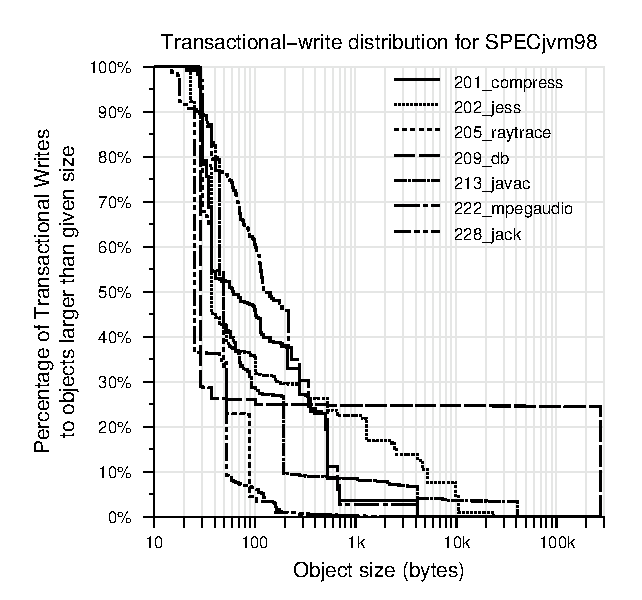
\includegraphics[width=2.25in,clip=true]{Figures/tr-w-all.eps}%
~~~~~%
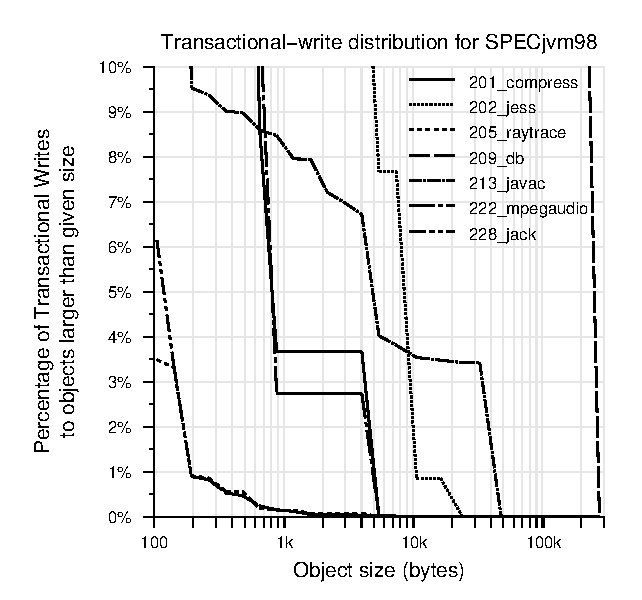
\includegraphics[width=2.25in,clip=true]{Figures/tr-w-ten.eps}%
\end{center}%
\caption{Proportion of transactional writes to objects equal to or
  smaller than a given size.  The right-hand graph zooms in on a
  portion of the relation shown in the left; note in particular that
  y-axis full-scale is only 10\% in the right-hand graph.}%
\label{fig:tr-w}%
\end{figure}%
Our software transactions implementation clones objects on
transactional writes, so that the previous state of the object can be
restored if the transaction aborts.  With this in mind, I was
interested in the number of writes to \emph{large} objects, or,
equivalently, on the object size distribution of transactional
writes.  \figref{tr-w} shows this distribution for the SPECjvm98
applications. 
}

\vspace*{5mm}

These preliminary results show that real applications can be
transactified with modest effort, yielding significant gains in
concurrency.  In other work \cite{AnanianAsKuLeLi04} we have shown
that a factor of 4 increase in concurrency can be obtained
by doing nothing more than converting locks to transactions.  Since
the transactified applications may contain large transactions,
proposed hardware support for transactions is inadequate.

%%%%%%%%%%%%%%%%%%%%%%%%%%%%%%%%%%%%%%%%%%%%%%%%%%%%%%%%%%%%%%%%%%
\section{Language-level Approaches to \\Synchronization}
\begin{figure}
{\it\sis%
\begin{tabular}{l}\sis%
{\bf const} myDirectory == {\bf object} oneEntryDirectory\\
~~{\bf export} Store, Lookup\\
~~{\bf monitor}\\
~~~~{\bf var} name : String\\
~~~~{\bf var} AnObject : Any\\
\\
~~~~{\bf operation} Store [ n : String, o : Any ]\\
~~~~~~name $\gets$ n\\
~~~~~~AnObject $\gets$ o\\
~~~~{\bf end} Store
\\
~~~~{\bf function} Lookup [ n : String ] $\to$ [ o : Any ]\\
~~~~~~{\bf if} n = name\\
~~~~~~~~{\bf then} o $\gets$ AnObject\\
~~~~~~~~{\bf else} o $\gets$ {\bf nil}\\
~~~~~~{\bf end if}\\
~~~~{\bf end} Lookup\\
\\
~~~~{\bf initially}\\
~~~~~~name $\gets$ {\bf nil}\\
~~~~~~AnObject $\gets$ {\bf nil}\\
~~~~{\bf end initially}\\
\\
~~{\bf end monitor}\\
{\bf end} oneEntryDirectory
\end{tabular}
}
\caption{A directory object in Emerald, from \cite{BlackHuJuLe86},
  illustrating the use of monitor synchronization.\index{monitor synchronization}}
\label{fig:emerald-dir}
\end{figure}

\begin{figure}
{\ttfamily\small\vspace{.25in}
\sis%
\begin{tabular}{l}
class Account \{\\
\\
~~int balance = 0;\\
\\
~~{\bf atomic} int deposit(int amt) \{\\
~~~~int t = this.balance;\\
~~~~t = t + amt;\\
~~~~this.balance = t;\\
~~~~return t;\\
~~\}\\
\\
~~{\bf atomic} int readBalance() \{\\
~~~~return this.balance;\\
~~\}\\
\\
~~{\bf atomic} int withdraw(int amt) \{\\
~~~~int t = this.balance;\\
~~~~t = t - amt;\\
~~~~this.balance = t;\\
~~~~return t;\\
~~\}\\
\\
\}\\
\end{tabular}
}\vspace{.2in}
\caption{A simple bank account object, adapted from \cite{FlanaganQa03},
  illustrating the use of the \atomic modifier.}
\label{fig:atomic}
\end{figure}

Our work on integrating transactions into the Java programming
language is related to prior work on integrating synchronization
mechanisms for multiprogramming, and in particular, to prior work on
synchronization in an object-oriented framework.

\index{Emerald|(}\label{sec:emerald}
The Emerald system \cite{BlackHuJuLe86,JulSt91} introduced
\defnlti{monitored objects} for synchronization.  Emerald code to
implement a simple directory object is shown in
Figure~\ref{fig:emerald-dir}.  Each object is associated with
Hoare-style monitor, which provides mutual exclusion and process
signalling.  Each Emerald object is divided into a monitored part and
a non-monitored part.  Variables declared in the monitored part are
shared, and access to them from methods in the non-monitored part is
prohibited---although non-monitored methods may call monitored methods
to effect the access.  Methods in the monitored part acquire the monitor lock
associated with the receiver object before entry and release it on
exit, providing for mutual exclusion and safe update of the shared
variables.  Monitored objects naturally integrate synchronization into
the object model.

Unlike Emerald monitored objects, where methods can only acquire the
monitor of their receiver and where restricted access to shared
variables is enforced by the compiler, Java implements a loose
variant where any monitor may be explicitly acquired and no shared
variable protection exists.  As a default, however, Java methods
declared with the {\tt synchronized} keyword behave like Emerald
monitored methods,
ensuring that the monitor lock of their receiver is held during execution.

Java's synchronization primitives arguably allow for more efficient
concurrent code than Emerald's---for example, Java objects can use
multiple locks to
protect disjoint sets of fields, and coarse-grain locks can be used
which protect multiple objects---but Java is also more prone to programmer
error.  However, even Emerald's restrictive
monitored objects are not sufficient to prevent data races.  As a
simple example, imagine that an object provided two monitored methods
{\tt read} and {\tt write} which accessed a shared variable.
Non-monitored code can call {\tt read}, increment the value returned,
and then call {\tt write}, creating a classic race condition scenario.
The atomicity of the parts is not sufficient to guarantee atomicity of
the whole \cite{FlanaganQa03}.
\note{``Composibility'': cite PPoPP paper?}
\index{Emerald|)}

This suggests that a better model for synchronization in
object-oriented systems is \defnlti{atomicity}.  Figure~\ref{fig:atomic}
shows Java extended with an \atomic keyword to implement an
object representing a bank account.  Rather than explicitly
synchronizing on locks, I simply require that the methods marked
\atomic execute atomically with respect to other threads in the
system; that is, that every execution of the program computes the same
result as some execution where all atomic methods were run \emph{in
  isolation} at a certain point in time, called the
\defni{linearization point}, between their invocation and return.
Note that
atomic methods invoked directly or indirectly from an atomic
method are subsumed by it: if the outermost method appears atomic,
then by definition all inner method invocations will also appear atomic.
Flanagan and Qadeer provide a more formal semantics in \cite{FlanaganQa03}.
Atomic methods can be analyzed using sequential reasoning techniques, which
significantly simplifies reasoning about program correctness.

Atomic methods can be implemented using locks.  A simple if inefficient
implementation would simply acquire a single global lock during
the execution of every atomic method.  Flanagan and Qadeer
\cite{FlanaganQa03} present a more sophisticated technique which proves that
a given implementation using standard Java monitors correctly
guarantees method atomicity.

The transaction implementations presented in this thesis will use
non-blocking synchronization to implement atomic methods.

\section{Related work}\label{sec:related}

A number of researchers have been investigating transactional memory
systems.  This thesis will be the first to present a model-checked non-blocking
object-oriented system which allows co-existence of non-transactional and
transactional accesses to a dynamic set of object fields.

\subsection{Non-blocking synchronization}\label{sec:nb-sync}

Lamport presented the first alternative to synchronization via mutual
exclusion in \cite{Lamport77}, for a limited situation involving a single
writer and multiple readers.  Lamport's technique relies on reading
guard elements in an order opposite to that in which they are written,
guaranteeing that a consistent data snapshot can be recognized.  The
writer always completes its part of the algorithm in a constant number
of steps; readers are guaranteed to complete only in the absence of
concurrent writes.

Herlihy formalized \emph{wait-free} implementations of
concurrent data objects in \cite{Herlihy88}.  A wait-free implementation
guarantees that any process can complete any operation in a finite
number of steps, regardless of the activities of other processes.
Lamport's algorithm is not wait-free
because readers can be delayed indefinitely.

Massalin and Pu introduced the term \emph{lock-free} to describe 
algorithms with weaker progress guarantees.
A lock-free implementation guarantees only that \emph{some}
process will complete in a finite number of steps
\cite{MassalinPu91}.  Unlike a wait-free implementation,
lock-freedom allows starvation.  Since other simple techniques can be
layered to prevent starvation (for example, exponential backoff),
simple lock-free implementations are usually seen as worthwhile practical
alternatives to more complex wait-free implementations.

An even weaker criterion, \emph{obstruction-freedom}, was introduced
by Herlihy, Luchangco, and Moir in \cite{HerlihyLuMo03}.
Obstruction-freedom only guarantees progress for threads executing in
isolation; that is, although other threads may have partially
completed operations, no other thread may take a step until the
isolated thread completes.  Obstruction-freedom not only allows
starvation of a particular thread, it allows contention among threads
to halt all progress in all threads
indefinitely.  External mechanisms are used to reduce contention
(thus, achieve progress) including backoff, queueing, or timestamping.

We will use the term \emph{non-blocking} to describe
generally any synchronization mechanism which doesn't rely on mutual
exclusion or locking, including wait-free, lock-free,
and obstruction-free implementations.
We will be concerned mainly with lock-free algorithms.%
\footnote{Note that some authors use ``non-blocking'' and
  ``lock-free'' as synonyms, usually meaning what we here call
  \emph{lock-free}.  Others exchange our definitions for ``lock-free''
  and ``non-blocking'', using lock-free as a generic term and non-blocking
  to describe a specific class of implementations.  As there is
  variation in the field, we choose to use the parallel construction
  \emph{wait-free}, \emph{lock-free}, and \emph{obstruction-free} for
  our three specific progress criteria, and the dissimilar
  \emph{non-blocking} for the general class.}

\subsection{Efficiency}\label{sec:efficiency}
Herlihy presented the first \emph{universal} method for wait-free
concurrent implementation of an arbitrary sequential object
\cite{Herlihy88,Herlihy91}.  This original method was based on
a \emph{fetch-and-cons} primitive, which atomically places
an item on the head of a list and returns the list of items following
it; all concurrent primitives capable of solving the
$n$-process consensus problem---\emph{universal} primitives---were
shown powerful enough to implement \emph{fetch-and-cons}.
In Herlihy's method, 
every sequential operation is translated into two steps.  In the first,
\emph{fetch-and-cons} is used to place the name and arguments of the
operation to be performed
at the head of a list, returning the other operations on the list.
Since the state
of a deterministic object is completely determined by the history of
operations performed on it, applying the operations returned
in order from last to first is sufficient to locally reconstruct the
object state 
prior to our operation.
We then use the prior state to compute the result of our operation
without requiring further synchronization with the other processes.

This first universal method was not very practical, a shortcoming
which Herlihy soon addressed \cite{Herlihy93}.  In addition, his revised universal
method can be made lock-free, rather than wait-free, resulting in
improved performance.  In the lock-free version of this method,
objects contain a shared variable
holding a pointer to their current state.  Processes begin by loading
the current state pointer and then copying the referenced state to a
local copy.  The sequential operation is performed on the
copy, and then if the object's shared state pointer is unchanged from
its initial load it is atomically swung to point at the updated state.

Herlihy called this the ``small object protocol'' because the object
copying overhead is prohibitive unless the object is small enough to
be copied efficiently (in, say, $O(1)$ time).  He also presented a
``large object protocol'' which requires the programmer to
manually break the object into small blocks, after which the small
object protocol can be employed. 
\punt{ This trouble with large objects is
common to many non-blocking implementations; our solution is presented
in \secref{proposal}.}

Barnes provided the first universal non-blocking implementation
method which avoids object copying \cite{Barnes93}.  He eliminates the
need to store ``old'' object
state in case of operation failure by having all threads cooperate to
apply operations.  For example, if the first processor begins an operation
and then halts, another processor will complete the operation of the first
before applying its own.  Barnes proposes to accomplish the
cooperation by creating a parallel state machine for each operation,
so that each thread can independently try to advance the machine from state
to state and thus advance incomplete operations.%
\footnote{It is interesting to note that Barnes' cooperative method
  for non-blocking 
  situation plays out in a real-time system very similarly to priority
  inheritance for locking synchronization.}
Although this avoids
copying state, the lock-step cooperative process is extremely
cumbersome and does not appear to have ever been implemented.
Furthermore, it does not protect against errors in the implementation
of the operations, which could cause \emph{every} thread to fail in turn
as one by one they attempt to execute a buggy operation.

Alemany and Felten \cite{AlemanyFe92} identified two factors hindering the
performance of non-blocking algorithms to date: resources wasted by operations
that fail, and the cost of data copying.  Unfortunately, they
proceeded to
``solve'' these problems by ignoring short delays and failures and
using operating system support to handle delays caused by
context switches, page faults, and
I/O operations.  This works in some situations, but obviously suffers
from a bootstrapping problem as the means to implement an operation system.

Although lock-free implementations are usually assumed to be more
efficient that wait-free implementations, LaMarca \cite{LaMarca94}
showed experimental evidence that Herlihy's simple
wait-free protocol scales very well on parallel machines.
When more than about twenty threads are involved, the wait-free
protocol becomes
faster than Herlihy's lock-free small-object protocol, three OS-aided
protocols of LaMarca and Alemany and Felten, and a
\emph{test-and-Compare\&Swap} spin-lock.

% Afek et al have a somewhat complicated improved wait-free method.

% Transactional memories?
\subsection{Transactional Memory Systems}\label{sec:tm}

Several software transaction systems have been proposed.  Some constrain the
programmer and make transactions difficult to use.  All have
relatively high overheads, which make transactions unattractive for
uniprocessor and small SMP systems. [Once the number of processors is
large enough, the increased parallelism which can be provided by
optimistic transactions may cancel out the performance penalty of
their use.]

The first proposal for software transactional memory was proposed by
Shavit and Touitou \cite{ShavitTo95}; their system requires that all
input and output locations touched by a transaction be known in
advance, which limits its application.  It performs at least 10
fetches and 4 stores per location accessed (not counting the loads and
stores directly required by the computation).  The benchmarks
presented were run on between 10 and 64 processors.

Rudys and Wallach \cite{RudysWa02} proposed a copying-based
transaction system to allow rollback of hostile codelets.
They show an order of magnitude slowdown for field and array
accesses, and 6x to 23x slowdown on their benchmarks.

Herlihy, Luchango, Moss, and Scherer's scheme \cite{HerlihyLuMoSc03}
allows transactions to touch a dynamic set of memory locations;
however the user still has to explicitly \emph{open} every object touched
before it can be used in a transaction.  This implementation is based
on object copying, and so has poor performance for large objects and
arrays.  Not including work necessary to copy objects involved in
writes, they require $O(R(R+W))$ work to open $R$ objects for reading
and $W$ objects for writing, which may be quadratic in the number of objects
involved in the transaction.   A list insertion benchmark which they
present shows 9x slowdown over a locking scheme, they beat the locking
implementation when more than 5-10 processors are active.  They
present benchmark data with up to 576 threads on 72 processors.

Harris and Fraser built a software transaction system on a flat
word-oriented transactional memory abstraction \cite{HarrisFr03},
roughly similar to simulating Herlihy's original hardware
transactional memory proposal in software.  This avoids problems with
large objects.  Performing $m$ memory operations touching $l$ distinct
locations costs at least $m+l$ extra reads and $l+1$ CAS operations, in
addition to the reads and writes required by the computation.
They appear to execute about twice as slowly as a locking
implementation on some microbenchmarks.  They benchmark on a
4-processor as well as a 106-processor machine; their crossover point
(at which the blocking overhead of locks matches the software
transaction overhead) is around 4 processors.
Note that Harris and Fraser do not address the problem of
concurrent non-transactional operations on locations involved in a
transaction.  Java synchronization allows such concurrent operations,
with semantics given by the Java memory model \cite{MansonPu02}.
We support these operations safely using our FLAG mechanism.

Programmers will be reluctant to use transactions to synchronize their
code when it results in their code running more slowly on the uniprocessor
and small-SMP systems which are most common today.
\note{Segue into hardware transactions writeup?}

Our preliminary work with SPECjvm98 and Linux case studies indicate that
transactional memory operations can be extremely common when
transactions are made easy to use and natural to express.  Programmers
can be expected to use both very small and very large transactions
when they are able, and transactions are used by the operating system
and programming libraries to provide synchronization and safety
properties.  Implementing transactional memory in hardware allows the
overheads to be low\note{\textbf{cite figures here}}, which is appropriate
when transactional operations are common.



%\chapter{An efficient software implementation of transactions}\label{cha:stm}
\section{Designing Efficient Transactions}\label{sec:efficient}
In this section I briefly describe some desired properties of the
software transaction system being designed for this thesis.

\subsection{Field Flags}\label{sec:flagfield}
\note{Missing: performance numbers for adding check.  Use ``no trans''
version of transaction app and add check into the access functions.}
We would like non-transactional code to execute with minimal overhead,
however, transactions should still appear atomic to non-transactional
code.  My basic mechanism is loosely based on the
distributed shared memory implementation of Scales and Gharachorloo
\cite{ScalesGh97}.  I pick a special ``flag'' value, and
``cross-out'' locations currently involved in a transaction by
overwriting them with the flag value.  Reading or attempting to
overwrite a flagged value will indicate to non-transactional code
that exceptional processing is necessary; all other non-transactional
operations proceed as usual.

Note that this technique explicitly allows safe access to fields
involved in a transaction from non-transactional code.
\punt{
Ensuring that transactional updates remain atomic to non-transactional
code eases ``transactification'' and 
Key idea is to allow safe access by non-transactional code, so as to
allow transactification.
}

\epsfigput{bloat}{Application slowdown with increasing object bloat
for the SPECjvm98 benchmark applications.}
\subsection{Object expansion}
I will need to add some additional information to each object to
track transaction state.  I measured the slowdown caused by various
amounts of object ``bloat'' to determine reasonable bounds on the
size of this extra information.  \figref{bloat} presents these
results for the SPECjvm98 applications; I determined that two words
(eight bytes) of additional storage per object would not impact
performance unreasonably.  This amount of bloat causes a geometric
mean of 2\% slowdown on these benchmarks.

\begin{figure}\sis%
\begin{center}
\begin{tabular}{lrrrr}
        & transactional & transactional\\
program & memory ops    & stores \% \\\hline
{\tt 201\_compress} & 50,029 & 26.2\% \\
{\tt 202\_jess} & 36,701,037 & 0.6\% \\
{\tt 205\_raytrace} & 7,294,648 & 23.2\% \\
{\tt 209\_db} & 195,374,420 & 6.3\% \\
{\tt 213\_javac} & 472,134,289 & 22.9\% \\
{\tt 222\_mpegaudio} & 41,422 & 18.6\% \\
{\tt 228\_jack} & 63,912,386 & 17.0\% \\
\end{tabular}
\end{center}
\caption{Comparison of loads and stores inside transactions for the
  SPECjvm98 benchmark suite, full input runs.}
\label{fig:writepercent}
\end{figure}
\subsection{Reads vs. Writes}
\figref{writepercent} shows that transactional reads typically
outnumber transactional writes by at least 4 to 1; in some cases reads
outnumber writes by over 100 to 1.  It is worthwhile, therefore, to
make reads more efficient than writes.  In particular, since the
flag-overwrite technique discussed in \secref{flagfield} requires us
to allocate additional memory to store the ``real'' value of the
field, I wish to avoid this process for transactional reads,
reserving the extra allocation effort for transactional writes.

\punt{
\subsection{Large objects}
See \secref{properties}.
}



\setlength{\epigraphwidth}{.4\textwidth}
\chapter{Transactions in hardware: Unbounded Transactional Memory}
\markboth{CHAPTER 6.~~TRANSACTIONS IN HARDWARE: UTM}{}
\label{cha:htm}\label{cha:hybrid}
\epigraphhead[70]{\epigraph{%
People who are really serious about software should make their own hardware.

Remember, it's all software, it just depends on when you crystallize
it.}{\textit{Alan Kay}}}
\index{Kay, Alan}
% http://www.folklore.org/StoryView.py?project=Macintosh&story=Creative_Think.txt

The previous chapters have detailed the design of an efficient
software-only transaction system for object-oriented programs.  Given
hardware support, we can construct even more efficient transaction
systems for certain types of transactions.  In this chapter, we will
present UTM, an implementation of unbounded transactional memory
\cite{AnanianAsKuLeLi04} which fully virtualizes transactions.  We
will follow this with LTM, a much simpler design which can be
pin-compatible with today's processors.  LTM supports more limited
transactions, but we conclude by showing how LTM can be combined with
the efficient software system we have already demonstrated to yield a
hybrid system with a great deal of power and
flexibility.\footnote{Portions of this chapter are adapted
from~\cite{AnanianAsKuLeLi04}, co-written with Krste Asanovi\'c,
Bradley C. Kuszmaul, Charles E. Leiserson, and Sean Lie.}

\section{The UTM architecture}\label{sec:utm}
We begin by describing UTM, a system that implements
unbounded transactional memory in hardware.  UTM allows
transactions to grow (nearly) as large as virtual memory.  It also
supports a semantics for nested transactions, where interior
transactions are subsumed into the atomic region represented by the
outer transaction.  Unlike previous schemes that tie a thread's
transactional state to a particular processor and/or cache, UTM
maintains bookkeeping information for a transaction in a
memory-resident data structure, the \defn{transaction log}.  This
enables transactions to survive timeslice interrupts and process
migration from one processor to another.  We first present the
software interface to UTM, and then describe the implementation
details.

\subsection{New instructions}

UTM adds two new instructions to a processor's instruction set
architecture:
\begin{description}
\item[\texttt{XBEGIN pc}:] Begin a new transaction.  The
\texttt{pc} argument to \texttt{XBEGIN} specifies
the address of an \defn{abort handler} (e.g., using a PC-relative offset).
If at any time during the execution of a transaction the hardware determines
that the transaction must fail, it immediately rolls back the
processor and memory state to what it was when \texttt{XBEGIN} was
executed, then jumps to \texttt{pc} to execute the abort handler.
 
\item[\texttt{XEND}:] End the current transaction.  If \texttt{XEND}
completes, then the transaction is committed, and all of its
operations appear to be atomic with respect to any other transaction.
\end{description}

Semantically, we can think of an \texttt{XBEGIN} instruction as a
conditional branch to the abort handler.  The \texttt{XBEGIN} for a
transaction that fails has the behavior of a mispredicted branch.
Initially, the processor executes the \texttt{XBEGIN} as a not-taken
branch, falling through into the body of the transaction.  Eventually
the processor realizes that the transaction cannot commit, at which
point it reverts all processor and memory state back to the point of
misprediction and branches to the abort handler.

In the same manner as our software implementation (\secref{withtrans}),
UTM supports the nesting of transactions by subsuming the inner
transaction.  For example, within an outer transaction, a
subroutine may be called that contains an inner transaction.
UTM simply treats the inner transaction as part of the atomic
region defined by the outer one.  This strategy is correct, because it
maintains the property that the inner transaction executes atomically.
Subsumed nested transactions are implemented by using a counter to
keep track of nesting depth.  If the nesting depth is positive, then
\texttt{XBEGIN} and \texttt{XEND} simply increment and decrement the
counter, respectively, and perform no other transactional bookkeeping.

\subsection{Rolling back processor state}

The branch mispredict mechanism in conventional superscalar processors
can roll back register state only for the small window of recent
instructions that have not graduated from the reorder buffer.  To
circumvent the window-size restriction and allow arbitrary rollback
for unbounded transactions, the processor must be modified to retain
an additional snapshot of the architectural register state.  A UTM
processor saves the state of its architectural registers when it
graduates an \texttt{XBEGIN}\@.  The snapshot is retained either until
the transaction aborts, at which point the snapshot is restored into
the architectural registers, or until the matching \texttt{XEND}
graduates indicating that the transaction has committed.

UTM's modifications to the processor core are illustrated in
\figref{snapshot}.  We assume a machine with a unified physical
register file, and so rather than saving the architectural registers
themselves, UTM saves a snapshot of the register-renaming table
and ensures the corresponding physical registers are not reused until
the transaction commits.
The rename stage maintains an additional ``saved'' bit
for each physical register 
to indicate which registers are part of the working
architectural state, and takes a snapshot as
each branch or \texttt{XBEGIN} is decoded and renamed.
When an \texttt{XBEGIN} instruction
graduates, activating the transaction, the associated ``\texttt{S} bit''
snapshot will have bits set
on exactly those registers holding the graduated architectural state.  Physical
registers are normally freed on graduation of a later instruction that
overwrites the same architectural register.  If the \texttt{S} bit on
the snapshot for the active transaction is
set, the physical register is added to a FIFO called a \defn{Register
Reserved List} instead of the normal \defn{Register Free List}.  This
prevents physical registers containing saved data from being
overwritten during a transaction.  When the
transaction's \texttt{XEND} commits, the active snapshot's \texttt{S}
bits are cleared and the Register
Reserved List is drained into the regular Register Free List.  In the
event that the transaction aborts, the saved register-renaming table
is restored and the reorder buffer is rolled back, as in an exception.
After restoring the architectural register state, the branch is taken
to the abort handler.  Even though the processor can internally
speculatively execute ahead through multiple transactions,
transactions only affect the global memory system as instructions
graduate, and hence UTM requires only a single snapshot of the
architectural register state.

The current transaction abort handler address, nesting depth, and
register snapshot are part of the transactional state.  They are made
visible to the operating system (as additional processor control
registers) to allow them to be saved and restored on context switches.

\subsection{Memory state}

Previous HTM systems \cite{Knight86,HerlihyMo93} represent a
transaction partly in the processor and partly in the cache, taking
advantage of the coincidence between the cache-consistency protocol
and the underlying consistency requirements of transactional memory.
Unlike those systems, UTM transactions are represented by a single
\defn{xstate} data structure held in the memory of the system.  The
cache in UTM is used to gain performance, but the correctness of
UTM does not depend on having a cache.  In the following
paragraphs, we first describe the xstate and how the system uses it
assuming there is no caching.  Then, we describe how caching
accelerates xstate operations.

The xstate is illustrated in \figref{datastruct-entry}.  The xstate
contains a transaction log for each active transaction in the system.
A transaction log is allocated by the operating system for each
thread, and two processor control registers hold the base and bounds
of the currently active thread's log.  Each log consists of a
\defn{commit record} and a vector of \defn{log entries}.  The commit
record maintains the transaction's status: \texttt{PENDING},
\texttt{COMMITTED}, or \texttt{ABORTED}.  Each log entry corresponds
to a block of memory that has been read or written by the transaction.
The entry provides a pointer to the block and the old (backup) value
for the block so that memory can be restored in case the transaction
aborts.  Each log entry also contains a pointer to the commit record
and pointers that form a linked list of all entries in all transaction
logs that refer to the same block.

The final part of the xstate consists of a \defn{log pointer} and one
\defn{RW bit} for each block in memory (and on disk, when paging).  If
the RW bit is \texttt{R}, any transactions that have accessed the
block did so with a load; otherwise, if it is \texttt{W}, the block
may have been the target of a transaction's store.  When a processor
running a transaction reads or writes a block, the block's log pointer
is made to point to a transaction log entry for that block.  Further,
if the access is a write, the RW bit for the block is set to
\texttt{W}.  Whenever another processor references a block that is
already part of a pending transaction, the system consults the RW bit
and log pointer to determine the correct action, for example, to use
the old value, to use the new value, or to abort the transaction.

\figput[UTM processor modifications.]{snapshot}%
{UTM processor modifications. The S bit vector
tracks the active physical registers.  For each rename table snapshot,
there is an associated S bit vector snapshot.  The Register Reserved
List holds the otherwise free physical registers until the transaction
commits.  The LPR field is the next physical register to free (the
last physical register referenced by the destination architectural
register).}

\figput[The xstate data structure.]{datastruct-entry}{%
The xstate data structure.
The transaction log for a transaction contains a commit record and a
vector of log entries.  The log pointer of a block in memory
points to a log entry, which contains the old value of the block and a
pointer to the transaction's commit record.  Two transaction logs
are shown here; generally, the xstate includes the active
transaction logs for the entire system.}

When a processor makes an update as part of a transaction, the new
value is stored in memory and the old value is stored in an entry in
the transaction log.  In principle, there is one log entry for every
load or store performed by the transaction.  If the memory allocated
to the log  is not large enough, the
transaction aborts and the operating system allocates a larger
transaction log and retries the transaction.  When
operating on the same block more than once in a transaction, the
system can avoid writing multiple entries into the transaction log by
checking the log pointer to see whether a log entry for the block
already exists as part of the running transaction.

By following the log pointer to the log entry, then following the log
entry pointer to the commit record, one can determine the transaction
status (pending, committed, or aborted) of each block.  To commit a
transaction, the system simply changes the commit record from
\texttt{PENDING} to \texttt{COMMITTED}.  At this point, a reference to
the block produces the new value stored in memory, albeit after some
delay in chasing pointers to discover that the transaction has been
committed.  To avoid this delay, as well as to free the transaction
log for reuse, the system must clean up after committing.  It does so
by iterating through the log entries, clearing the log pointer for
each block mentioned, thereby finalizing the contents of the block.
Future references to that block will continue to produce the new value
stored in memory, but without the delay of chasing pointers.  To abort
a transaction, the system changes the commit record from
\texttt{PENDING} to \texttt{ABORTED}.  To clean up, it iterates
through the entries, storing the old value back to memory and then
clearing the log pointer.  We chose to store the old value of a block
in the transaction log and the new value in memory, rather than the
reverse, to optimize the case when a transaction commits.  No data
copying is needed to clean up after a commit, only after an abort.

When two or more pending transactions have accessed a block and at
least one of the accesses is a store, the transactions conflict.
Conflicts are detected during operations on memory.  When a
transaction performs a load, the system checks that either the log
pointer refers to an entry in the current transaction log, or else
that the RW bit is \texttt{R} (additionally creating an entry in the
current log for the block if needed).  When a transaction performs a
store, the system checks that no other transaction is referenced by
the log pointer (i.e., that the log pointer is cleared or that the
linked list of log entries corresponding to this block are all
contained in the current transaction log).  If the conflict check
fails, then some of the conflicting transactions are aborted.  To
guarantee forward progress, UTM writes a timestamp into the
transaction log the first time a transaction is attempted.  Then, when
choosing which transactions to abort, older transactions take
priority.  As an alternative, a backoff scheme \cite{MetcalfeBo76}
could also be used.

When a writing transaction wins a conflict, there may be multiple
reading transactions that must be aborted.  These transactions are
found efficiently by following the block's log pointer to an entry and
traversing the linked list found there, which enumerates all entries
for that block in all transaction logs.

\subsection{Caching}

Although UTM can support transactions of unbounded size using the
xstate data structure, multiple memory accesses for each operation may
be required.  Caching is needed to achieve acceptable performance.  In
the common case of a transaction that fits in cache, UTM, like the
earlier proposed HTM systems \cite{Knight86,HerlihyMo93}, monitors the
cache-coherence traffic for the transaction's cache lines to determine
if another processor is performing a conflicting operation.  For
example, when a transaction writes to a memory location, the cache
protocol obtains exclusive ownership on the whole cache block.  New
values can be stored in cache with old values left in memory.  As long
as nothing revokes the ownership of any block, the transaction can
succeed.  Since the contents of the transaction log are undefined
after the transaction commits or aborts, in many cases the system does
not even need to write back a transaction log.  Thus, for a small
transaction that commits without intervention from another
transaction, no additional interprocessor communication is required
beyond the coherence traffic for the nontransactional case.  When the
transaction is too big to fit in cache or interactions with other
transactions are indicated by the cache protocol, the xstate for the
transaction overflows into the ordinary memory hierarchy.  Thus, the
UTM system does not actually need to create a log entry or update
the log pointer for a cached block unless it is evicted.  After a
transaction commits or aborts, the log entries of unspilled cached
blocks can be discarded and the log pointer of each such block can be
marked clean to avoid writeback traffic for the log pointer, which is
no longer needed.  Most of the overhead is borne in the uncommon case,
allowing the common case to run fast.

The in-cache representation of transactional state and the xstate data
structure stored in memory need not match.  The system can optimize
the on-processor representation as long as, at the cache interface, the
view of the xstate is properly maintained.  For convenience, the
transaction block size can match the cache line size.

\subsection{System issues}

The goal of UTM is to support transactions that can run for an
indefinite length of time (surviving time slice interrupts), can
migrate from one processor to another along with the rest of a
process's state, and can have footprints bigger than the physical
memory.  Several system issues must be solved for UTM to achieve that
goal.  The main technique that we propose is to treat the xstate as
a system-wide data structure that uses global virtual addresses.

Treating the xstate as data structure directly solves part of the
problem.  For a transaction to run for an indefinite length of time,
it must be able to survive a time-slice interrupt.  By adding the
log pointer to the processor state and storing everything else in a
data structure, it is easy to suspend a transaction and run another
thread with its own transaction.  Similarly, transactions can be
migrated from one processor to another.  The log pointer is
simply part of the thread or process state provided by the operating
system.

UTM can support transactions that are even larger than physical
memory.  The only limitation is how much virtual memory is available
to store both old and new values.  To page the xstate out of main
memory, the UTM data structures might employ global virtual addresses for
their pointers.  Global virtual addresses are system-wide unique
addresses that remain valid even if the referenced pages are paged out
to disk and reloaded in another location.  Typically, systems that
provide global virtual addresses provide an additional level of
address translation, compared to ordinary virtual memory systems.
Hardware first translates a process's virtual address into a global
virtual address.  The global virtual address is then translated into a
physical address.  Multics \cite{BensoussanClDa72} provided user-level
global virtual addressing using segment-offset pairs as the addresses.
The HP Precision Architecture \cite{Lee89} supports global virtual
addresses in a 64-bit RISC processor.

The log pointer and state bits for each user memory block,
while typically not visible to a user-level programmer, are
themselves stored in addressable physical memory to allow the
operating system to page this information to disk.  The location of
the memory holding the log pointer information for a given user data
page is kept in the page table and cached in the TLB.

During execution of a single load or store instruction, the processor can
potentially touch a large number of disparate memory locations in the
xstate, any of which may be paged out to disk.  To ensure forward
progress, either the system must allow load or store instructions to
be restarted in the middle of the xstate traversal, or, if only
precise interrupts are allowed, the operating system must ensure that
all pages required by an xstate traversal can be resident
simultaneously to allow the load or store to complete without page
faults.

UTM assumes that each transaction is a serial instruction stream
beginning with an \texttt{XBEGIN} instruction, ending with a
\texttt{XEND} instruction, and containing only register, memory, and
branch instructions in between.  A fault occurs if an I/O instruction
is executed during a transaction.

\section{The LTM architecture}\label{sec:ltm}

UTM is an idealized design for HTM that requires significant
changes to both the processor and the memory subsystem of a current
computer architecture.  By scaling back on the degree of
``unboundedness,'' however, a compromise between programmability and
practicality can be achieved.  This section presents such an
architectural compromise, called LTM, for which we have implemented
a detailed cycle-level simulation using UVSIM~\cite{Zhang03}.
The limited transactions supported by LTM are still powerful enough to
serve as the basic for an hybrid system, as we will show in
\secref{hybrid}.

LTM's design is easier to implement than UTM, because it does
not support transactions of virtual-memory size.  Instead, LTM
avoids the intricacies of virtual memory by limiting the footprint of
a transaction to (nearly) the size of physical memory.  In addition,
the duration of a transaction must be less than a time slice and
transactions cannot migrate between processors.  With these
restrictions, LTM can be implemented by only modifying the cache
and processor core and without making changes to the main memory, the
cache-coherence protocols, or even the contents of the cache-coherence
messages.  Unlike a UTM processor, an LTM processor can be
pin-compatible with a conventional processor.  The design presented
here is based on the SGI Origin 3000 shared-memory multiprocessor,
with memory distributed among the processor nodes and cache coherency
maintained using a directory-based write-invalidate protocol.

The UTM and LTM schemes share many ideas.  Like UTM, LTM
maintains data about pending transactions in the cache and detects
conflicts using the cache-coherency protocol in much the same way as
previous HTM proposals~\cite{Knight86, HerlihyMo92}.  LTM also employs an
architectural state-save mechanism in hardware.  Unlike UTM, LTM
does not treat the transaction as a data structure.  Instead, it binds
a transaction to a particular cache.  Transactional data overflows
from the cache into a hash table in main memory, which allows LTM
to handle transactions too big to fit in the cache without the
full implementation complexity of the xstate data structure.

LTM has similar semantics to UTM, and the format and behavior of
the \texttt{XBEGIN} and \texttt{XEND} instructions are the same.
The information that UTM keeps in the transaction log is
kept partly in the processor, partly in the cache, and partly in an
area of physical memory allocated by the operating system.

\figput[LTM cache modifications.]{cachemods}{LTM cache modifications. The T bit indicates if the line is
transactional. The O bit indicates if the set has
overflowed. Overflowed data is stored in a data structure in uncached
DRAM.}

LTM requires only a few small modifications to the cache, as shown
in \figref{cachemods}.  For small transactions, the cache is used to
store the speculative transactional state. For large transactions,
transactional state is spilled into an overflow data structure in main
memory. An additional bit (T) is added per cache line to indicate if
the data has been accessed as part of a pending transaction. When a
transactional-memory request hits a cache line, the T bit is set. An
additional bit (O) is added per cache set to indicate if it has
overflowed. When a transactional cache line is evicted from the cache
for capacity reasons, the O bit is set.

In LTM, the main memory always contains the original state of any
data being modified transactionally, and all speculative transactional
state is stored in the cache and overflow hash table.  A transaction
is committed by simply clearing all the T bits in cache and writing
all overflowed data back to memory. Conflicts are detected using the
cache-coherency protocol.  When an incoming cache intervention hits a
transactional cache line, the running transaction is aborted by simply
clearing all the T bits and invalidating all modified transactional
cache lines.
\note{CSA: I presume we NACK any cache intervention while we're writing
the overflow table back to memory?}

The overflow hash table in uncached main memory is maintained by
hardware, but its location and size are set up by the operating
system.  If a request from the processor or a cache intervention
misses on the resident tags of an overflowed set, the overflow hash
table is searched for the requested line.  If the requested cache line
is found, it is swapped with a line in the cache set and handled like
a hit.  If the line is not found, it is handled like a miss.  While
handling overflows, all incoming cache interventions are stalled using
a NACK-based network protocol.

The LTM overflow data structure uses the low-order bits of the address
as the hash index and uses linear probing to resolve conflicts.  When
the overflow data structure is full, the hardware signals an exception
so that the operating system can increase the size of the hash table
and retry the transaction.

LTM was designed to be a first step towards a truly unbounded
transactional memory system such as UTM.  LTM has most of the
advantages of UTM while being much easier to implement.  As I will
show at the end of the chapter, LTM's
more practical implementation of quasi-unbounded transactional memory
suffices for many real-world concerns, and can be symbiotically paired
with our more flexible software transaction system to achieve truely
unbounded transactions at minimal hardware cost.

%%%%%%%%%%%%%%%%%%%%%%%%%%%%%%%%%%%%%%%%%%%%%%%%%%%%%%%%%
\section{Evaluation}\label{sec:htm-benchmarks}
In this section we will evaluate the UTM and LTM designs,
demonstrating low overhead and scalability.  We will also
consider overflow behavior, providing some motivation for the hybrid
system proposed in the next section.

\subsection{Scalability}\label{sec:htm-counter}

\begin{figure}
\begin{center}
\begin{tabular}{c}
\includegraphics{Figures/uvsimCounterRuntime}
%% \includegraphics{uvsimLinkedListRuntime.eps}
\end{tabular}
\end{center}
\caption{\texttt{Counter} performance on UVSIM.}
\label{fig:microbenchperf}
\end{figure}

We used a parallel microbenchmark to examine
program behavior for small transactions with high contention. Our
results show that the extremely low overhead of small hardware transactions
enable them to almost always complete even when contention is high.

The \texttt{Counter} microbenchmark has one shared variable that each
processor atomically increments repeatedly with no backoff
policy; the basic idea is identical to the microbenchmark we used in
\secref{counter-bench}.
Each transaction is only a few instructions long and every
processor attempts to write to the same location repeatedly.  Both a
locking and a transactional version of \texttt{Counter} were run on
UVSIM with LTM, and the results are shown in
\figref{microbenchperf}. In the locking version, there is a global
spin-lock that each processor obtains using a
load-linked/store-conditional (LLSC) sequence from the SGI
synchronization libraries.

The locking version scales poorly, because the LLSC causes many cache
interventions even when the lock cannot be obtained. On the other
hand, the transactional version scales much better, despite having no
backoff policy.  When a transaction obtains a cache line, it is likely
to be able to execute a few more instructions before receiving an
intervention since the network latency is high.  Therefore, small
transactions can start and complete (and perhaps even start and
complete the next transaction) before the cache line is taken away.
Similar behavior is expected from UTM, and other transactional-memory
systems that use the cache and cache-coherency protocol to store
transactional state, since small transactions effectively use the
cache the same way. 

\subsection{Overhead}

A main goal of LTM and UTM is to run the common case fast. As shown in
\secref{properties}, the common case is when transactions are small
and fit in the cache. Therefore, by using the cache and cache
coherency mechanism to handle small transactions, LTM is able to
execute with almost no overhead over serial code in the common
case. In this section, we discuss qualitatively how the LTM
implementation is optimized for the common case and how similar
techniques are used in UTM. The discussion is broken into the
following three cases: starting, running, committing a transaction.

Starting a transaction in LTM requires virtually no overhead in the
common case since the hardware only needs to record the abort handler
address. No communication with the cache or other external hardware is
necessary. There is the added overhead of decoding the \texttt{XBEGIN}
however that overhead is generally insignificant compared to the cost
of the transaction. Further, instruction decode overhead is much lower
in LTM than with locks. Even schemes where the lock is not actually
held such as SLE~\cite{RajwarGo01} have higher decode overhead since they have more
instructions. LTM's low transaction startup overhead is a very good
indicator of the corresponding overhead in UTM since transaction start
up in UTM is virtually the same.

Running a transaction in LTM requires no more overhead than running
the corresponding non-synchronized code in the common case. In LTM,
the T bit is simply set on each transactional cache access. LTM's low
overhead in this case unfortunately does not translate directly to UTM
since UTM modifies the transaction record on each memory
request. However, in the common case the transaction record entry is
also in the cache. Thus all operations are local and no external
communication is needed. Also, in some cases, the cache can respond to
the memory request once the requested data is found. However, if the
request requires data from the transaction record before it can be
serviced, an additional cache lookup is necessary. However, the lookup
is local and thus can be done relatively quickly. \note{Is this
enough?  Seems like the additional lookup in the cache could increase
cache latency significantly} Therefore, the common case overhead of
running a transaction can be minimal even in UTM.

Committing a transaction in LTM has virtually no overhead in the
common case since it can be done in one clock cycle. LTM transaction
commits only requires a simply flash clear of all the transaction bits
in the cache. Similarly, UTM transaction commits only require a single
change of the cached transaction record to ``committed''. UTM
transaction commit also writes the updated values from the transaction
record back to memory. However, this write back can be done lazily in
the background.  Therefore, since transaction commit requires only a
single change in the cache for both LTM and UTM, the overhead is
minimal in both cases.

\subsection{Overflows}

Overflows occur only in the uncommon case
however our studies show that it is important to have a scalable data
structure even though it is used infrequently.

For evaluation, we compiled three versions of the SPECjvm98 benchmark
suite to run under UVSIM using FLEX. We compiled
a \defn{Base} version that uses no synchronization, a \defn{Locks}
version that uses spin-locks for synchronization, and a \defn{Trans}
version that uses LTM transactions for synchronization. To measure
overheads, we ran these versions of the SPECjvm98 benchmark suite on
one processor of UVSIM.

As described in \secref{synctrans}, our transactional version uses method
cloning to flatten transactions; we performed the same cloning on the
other compiled versions so that performance improvements due to the
specialization would not be improperly attributed to
transactionification.  The three different benchmark versions were
built from a common code-base using method inlining in \texttt{gcc}\footnote{We
compiled the files generated by FLEX's ``Precise C'' backend
(\secref{precisec}) with
\texttt{-O9} for a \texttt{-mips4} target using the
\texttt{n64} API to generate fully-static binaries executable by
UVSIM.}  to remove or replace all invocations of lock and transaction
entry and exit code with appropriate implementations.  No garbage
collection was performed during these benchmark runs.

\label{sec:javac}
Our initial results from \secref{properties} suggested that
overflows ought to be infrequent, thus the efficiency of the overflow
data structure would 
have a negligible effect on overall performance. Therefore, our first
LTM implementation used an unsorted array that required a linear
search on each miss to an overflowed set. The unsorted array was
effective for most of our test cases, as they had less overhead than
locks.  Using LTM with the unsorted array, however, the transactional
version of \texttt{213\_javac} was 14 times slower than the base
version.  Virtually all of the overhead came from handling overflows,
which is not surprising, since the entire application is enclosed in
one large transaction. The large transaction touches 13K cache lines
with 9K lines overflowed.  So, even though only 0.5\% of the
transactional memory operations miss in the cache, each one incurs a
huge search cost. This unexpected slowdown indicated that a naive
unsorted array is insufficient as an overflow data
structure. Therefore, LTM was redesigned to use a hash table to store
overflows.

Since the entire application was enclosed in a transaction, the
\texttt{213\_javac} application was clearly not written to be a
parallel application. However, it is important that an unbounded
transactional memory system be able to support even such applications
with reasonable performance. Therefore, we redesigned LTM to use hash
table as described in \secref{ltm}.


\begin{figure}
\footnotesize
\begin{center}
\begin{tabular}{l|r|rr|rr}
Benchmark                 &  Base       & Locks         & Trans                  & Time in   & Time in                    \\
application               &  time       & time          & time                   & trans     & overflow                   \\
                          &  (cycles)   & \multicolumn{2}{c|}{(\% of Base time)} & \multicolumn{2}{c}{(\% of Trans time)} \\ \hline
\texttt{200\_check}       &   8.1M      & 124.0\%       & 101.0\%                & 32.5\%     & 0.0085\%                  \\
% \texttt{201\_compress}    & 608.3M      & 102.5\%       & 106.1\%                &  3.8\%     & 4.0\%                     \\
\texttt{202\_jess}        &  75.0M      & 140.9\%       & 108.0\%                & 59.4\%     & 0.0072\%                  \\
\texttt{209\_db}          &  11.8M      & 142.4\%       & 105.2\%                & 54.0\%     & 0\%                       \\
\texttt{213\_javac}       &  30.7M      & 169.9\%       & 114.2\%                & 84.2\%     & 10\%                      \\
\texttt{222\_mpegaudio}   &  99.0M      & 100.3\%       &  99.6\%                &  0.8\%     & 0\%                       \\
\texttt{228\_jack}        & 261.4M      & 175.3\%       & 104.3\%                & 32.1\%     & 0.0056\%                  \\
\end{tabular}
\end{center}
\caption[SPECjvm98 performance on a 1-processor UVSIM simulation.]{%
SPECjvm98 performance on a 1-processor UVSIM simulation.  The {\em
Time in trans} and {\em Time in overflow} are the times spent actually
running a transaction and handling overflows respectively. The input
size is 1. The overflow hash table is 128MB.}
\label{fig:specperf}
\end{figure}

Using LTM with the hash table, the SPECjvm98 application overheads
were much more reasonable as shown in \figref{specperf}.  The hash
table data structure decreased the overhead from a 14x slowdown to
under 15\% in \texttt{213\_javac}. Using the hash table, LTM
transactional overhead is less than locking overhead in all cases.

%%%%%%%%%%%%%%%%%%%%%%%%%%%%%%%%%%%%%%%%%%%%%%
\punt{
These results indicate that UTM will also have minimal overhead, since
the UTM data structure behaves much like the LTM hash table. When we
miss in the cache, LTM requires one additional access of memory to
index the hash table when there is no conflict. Similarly, UTM
requires one additional access of memory to retrieve the requested
cache line.  UTM may require an additional access of memory, however,
to retrieve the transactional record entry. UTM requires at most one
more access to memory than LTM when there is overflow.  Therefore, the
overflow overhead of UTM will be very similar to that of UTM.
}



\punt{
\section{Evaluation}
\section{Making UTM fast}
% describe how caching works.

% Extending Transactions: beyond atomic power.
\section{Extending hardware transactions}\label{sec:htmplus}
\subsection{Nesting}
\subsection{Exchange and merging}
\subsection{Loopholes and NITs}\label{sec:nit}
\subsection{Opportunistic parallelism}

%%%%%%%%%% Extending the hardware section %%%%%%%%%%555

% First: do we want to?  Next section should how to make software hybrid.

\section{Adding partial rollback}
\subsection{LTM}
% keep a log(n) bit 'nesting level' with each transaction
% bulk decremember nesting level on commit.
% is this really needed?  Why not just 'checkpoints'?
% numbering system: what we really want to do is breadth-first
% numbering of the tree, so that we have well-spaced checkpoints.

\subsection{UTM}
% think about implications here.

\section{Making abort handlers more general}
% calling-convention and function issues.
% save registers in software
% do aborts in software
% this lets us add custom compensation code.
% what environment?  just pick one.

%% Extending Transactions: beyond atomic power.
%\section{Nesting}
%\section{Exchange and merging}
%\section{Loopholes and NITs}\label{sec:nit}
%\section{Opportunistic parallelism}

% LocalWords:  UTM XBEGIN XEND mispredicted misprediction superscalar Herlihy
% LocalWords:  mispredict LTM UVSIM SGI transactionally uncached lookup SPECjvm
% LocalWords:  inlining microbenchmark xstate RW RISC

\section{A Real Implementation}
Some notes about a ``real'' implementation of UTM.

MIPS.  Let's assume a primary cache line of 16 bytes, and a secondary
cache line of 128 bytes.  Our transaction block size will be the same
as the secondary cache line size, 128-bytes, which will limit our
address-space overhead to approximately 8\%.  The transaction data (descriptor)
associated with a block will fit into 8 bytes (one 64-bit word), since
virtual addresses are limited to 40 bits on MIPS (42 if you include
the kernel/supervisor/user mode bits; AMD-64 has 52-bit virtual
addresses).\footnote{A(63:62)=$10_2$ is not currently used; we could
steal this to indicate ``transaction descriptors''.  This would probably
cause protection problems.}

There would be 16 transaction descriptor words on a cache line; this
could cause ping-ponging.  An 8k page contains descriptors for the
transaction blocks on 16 other pages ($2^10$ descriptors).  The
descriptors should be arranged so the ``no information'' is an
all-zeros pattern.  The OS can then garbage collect any transaction
descriptor pages which contain all zeros (instead of eg paging them to
disk; I believe most OSes will do this optimization already, but maybe
not if the page was once dirty).\footnote{Alternatively, we could reference
count these pages in the page table, and deallocate them when the
number of non-zero entries on the page drops to zero.  This is
probably not the best way to do it.}

To find the transaction descriptor for a given virtual address, we
just flip a high-order bit and shift the low-order bits.  This reuses
the TLB, etc, mechanisms for virtualization, but we must be careful
that we can still ensure forward progress and don't introduce spurious
transaction performance conflicts (because transaction descriptors for
two different transactions reside on the same cache line).

The caches need to know the details of these 'special' addresses so
that ``on chip'' transactions are handled correctly.  In fact, the
cache organization would probably look more like the figure (with the
information stored alongside the cache lines), and we might want to
have extra cache-associativity or other mechanisms to prevent
ping-ponging of the transaction descriptors. (Is this right?)


Another alternative: 9-bit bytes would give enough transaction
descriptor info for 64-byte transaction blocks.

}

\begin{figure}[t]\begin{center}%
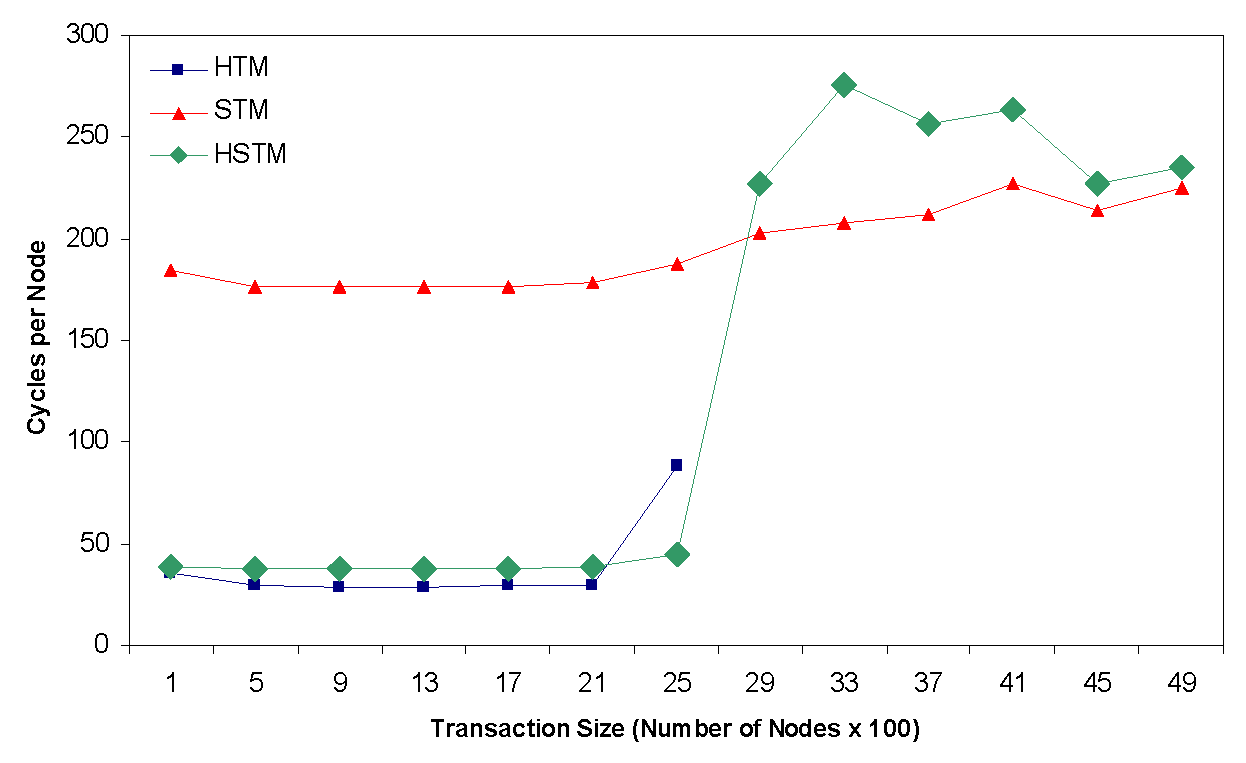
\includegraphics[width=3.25in,clip=true]{Figures/sean_lie_6b.eps}%
\end{center}%
\caption{Performance (in cycles per node push on a simple queue
  benchmark) of LTM~\cite{AnanianAsKuLeLi04} (HTM), the
  object-based system presented in this paper (STM) and a hybrid
  scheme (HSTM).}%
\label{fig:hybrid}%
\end{figure}
It is worth considering if a low-level HTM can yield benefits other
than efficient implementations of large-object operations.  In fact,
\figref{hybrid} presents research showing that we can combine the
strengths of our object-based software transaction system with a
fast bounded-size HTM.  In the figure, combining the systems is done
in the most simple-minded way: all transactions are begun in
LTM~\cite{AnanianAsKuLeLi04},
and after any abort the transaction is restarted in the
object-based software system.  The field flag mechanism described in
\secref{flagfield} ensures that software transactions properly abort
conflicting hardware transactions; hardware transactions must perform
the \texttt{ReadNT} and \texttt{WriteNT} algorithms for a slight
overhead (as shown in the figure).


\punt{
\chapter{Extending the hardware}\label{cha:htmplus}
\epigraphhead[70]{\epigraph{%
To create a new standard, it takes something that's not just a little
bit different; it takes something that's really new and really
captures people's imagination\ldots.}{\textit{Bill Gates}, 1984.}}
%%%%%%%%%% Extending the hardware section %%%%%%%%%%555

% First: do we want to?  Next section should how to make software hybrid.

\section{Adding partial rollback}
\subsection{LTM}
% keep a log(n) bit 'nesting level' with each transaction
% bulk decremember nesting level on commit.
% is this really needed?  Why not just 'checkpoints'?
% numbering system: what we really want to do is breadth-first
% numbering of the tree, so that we have well-spaced checkpoints.

\subsection{UTM}
% think about implications here.

\section{Making abort handlers more general}
% calling-convention and function issues.
% save registers in software
% do aborts in software
% this lets us add custom compensation code.
% what environment?  just pick one.

%% Extending Transactions: beyond atomic power.
%\section{Nesting}
%\section{Exchange and merging}
%\section{Loopholes and NITs}\label{sec:nit}
%\section{Opportunistic parallelism}

}

\punt{
\epigraphhead[70]{\epigraph{%
Hybrids are often named by the portmanteau method, combining the names
of the two parent species. For example, a zeedonk is a cross between a
zebra and a donkey.}{\textit{Wikipedia}, ``Hybrid''}}

% dual-path coding: publishable paper: try in hw, fall back to software


\chapter{Compiler optimizations and type systems}
% Optimizations and type systems.
\section{Closing the semantic gap}\label{sec:safe-transactify}

}

% 'Challenges' chapter.
\section{Performance isolation}
\note{Cite WDDD here.}
\section{Progress guarantees}\label{sec:progress}
\section{The semantic gap}\label{sec:semantic}
\section{I/O}
\section{OS interactions}


\chapter{Related work}\label{cha:related}
\epigraphhead[70]{\epigraph{%
Everything in the universe relates to [transactions], one way or another,
given enough ingenuity on the part of the interpreter.
}{\textit{Principia Discordia} (amended)}}

A number of researchers have been investigating transactional memory
systems.  This thesis is the first to present a hybrid hardware/software
model-checked non-blocking
object-oriented system that allows co-existence of non-transactional and
transactional accesses to a dynamic set of object fields.
\note{Martin wants citations here: ask him about this?}

\section{Non-blocking synchronization}\label{sec:nb-sync}

Lamport presented the first alternative to synchronization via mutual
exclusion in \cite{Lamport77}, for a limited situation involving a single
writer and multiple readers.  Lamport's technique relies on reading
guard elements in an order opposite to that in which they are written,
guaranteeing that a consistent data snapshot can be recognized.  The
writer always completes its part of the algorithm in a constant number
of steps; readers are guaranteed to complete only in the absence of
concurrent writes.

Herlihy formalized \emph{wait-free} implementations of
concurrent data objects in \cite{Herlihy88}.  A wait-free implementation
guarantees that any process can complete any operation in a finite
number of steps, regardless of the activities of other processes.
Lamport's algorithm is not wait-free
because readers can be delayed indefinitely.

Massalin and Pu introduced the term \emph{lock-free} to describe 
algorithms with weaker progress guarantees.
A lock-free implementation guarantees only that \emph{some}
process will complete in a finite number of steps
\cite{MassalinPu91}.  Unlike a wait-free implementation,
lock-freedom allows starvation.  Since other simple techniques can be
layered to prevent starvation (for example, exponential backoff),
simple lock-free implementations are usually seen as worthwhile practical
alternatives to more complex wait-free implementations.

An even weaker criterion, \emph{obstruction-freedom}, was introduced
by Herlihy, Luchangco, and Moir in \cite{HerlihyLuMo03}.
Obstruction-freedom only guarantees progress for threads executing in
isolation; that is, although other threads may have partially
completed operations, no other thread may take a step until the
isolated thread completes.  Obstruction-freedom not only allows
starvation of a particular thread, it allows contention among threads
to halt all progress in all threads
indefinitely.  External mechanisms are used to reduce contention
(thus, achieve progress) including backoff, queueing, or timestamping.

We will use the term \emph{non-blocking} to describe
generally any synchronization mechanism that doesn't rely on mutual
exclusion or locking, including wait-free, lock-free,
and obstruction-free implementations.
We will be concerned mainly with lock-free algorithms.%
\footnote{Note that some authors use ``non-blocking'' and
  ``lock-free'' as synonyms, usually meaning what we here call
  \emph{lock-free}.  Others exchange our definitions for ``lock-free''
  and ``non-blocking'', using lock-free as a generic term and non-blocking
  to describe a specific class of implementations.  As there is
  variation in the field, we choose to use the parallel construction
  \emph{wait-free}, \emph{lock-free}, and \emph{obstruction-free} for
  our three specific progress criteria, and the dissimilar
  \emph{non-blocking} for the general class.}

\section{Efficiency}\label{sec:efficiency}
Herlihy presented the first \emph{universal} method for wait-free
concurrent implementation of an arbitrary sequential object
\cite{Herlihy88,Herlihy91}.  This original method was based on
a \emph{fetch-and-cons} primitive, which atomically places
an item on the head of a list and returns the list of items following
it; all concurrent primitives capable of solving the
$n$-process consensus problem---\emph{universal} primitives---were
shown powerful enough to implement \emph{fetch-and-cons}.
In Herlihy's method, 
every sequential operation is translated into two steps.  In the first,
\emph{fetch-and-cons} is used to place the name and arguments of the
operation to be performed
at the head of a list, returning the other operations on the list.
Since the state
of a deterministic object is completely determined by the history of
operations performed on it, applying the operations returned
in order from last to first is sufficient to locally reconstruct the
object state 
prior to our operation.
We then use the prior state to compute the result of our operation
without requiring further synchronization with the other processes.

This first universal method was not very practical, a shortcoming
which Herlihy soon addressed \cite{Herlihy93}.  In addition, his revised universal
method can be made lock-free, rather than wait-free, resulting in
improved performance.  In the lock-free version of this method,
objects contain a shared variable
holding a pointer to their current state.  Processes begin by loading
the current state pointer and then copying the referenced state to a
local copy.  The sequential operation is performed on the
copy, and then if the object's shared state pointer is unchanged from
its initial load it is atomically swung to point at the updated state.

Herlihy called this the ``small object protocol'' because the object
copying overhead is prohibitive unless the object is small enough to
be copied efficiently (in, say, $O(1)$ time).  He also presented a
``large object protocol'' which requires the programmer to
manually break the object into small blocks, after which the small
object protocol can be employed. 
[This trouble with large objects is
common to many non-blocking implementations; our solution is presented
in \charef{largeobj}.]

Barnes provided the first universal non-blocking implementation
method that avoids object copying \cite{Barnes93}.  He eliminates the
need to store ``old'' object
state in case of operation failure by having all threads cooperate to
apply operations.  For example, if the first processor begins an operation
and then halts, another processor will complete the operation of the first
before applying its own.  Barnes proposes to accomplish the
cooperation by creating a parallel state machine for each operation,
so that each thread can independently try to advance the machine from state
to state and thus advance incomplete operations.%
\footnote{It is interesting to note that Barnes' cooperative method
  for non-blocking 
  situation plays out in a real-time system very similarly to priority
  inheritance for locking synchronization.}
Although this avoids
copying state, the lock-step cooperative process is extremely
cumbersome and does not appear to have ever been implemented.
Furthermore, it does not protect against errors in the implementation
of the operations, which could cause \emph{every} thread to fail in turn
as one by one they attempt to execute a buggy operation.

Alemany and Felten \cite{AlemanyFe92} identified two factors hindering the
performance of non-blocking algorithms to date: resources wasted by operations
that fail, and the cost of data copying.  Unfortunately, they
proceeded to
``solve'' these problems by ignoring short delays and failures and
using operating system support to handle delays caused by
context switches, page faults, and
I/O operations.  This works in some situations, but obviously suffers
from a bootstrapping problem as the means to implement an operating system.

Although lock-free implementations are usually assumed to be more
efficient that wait-free implementations, LaMarca \cite{LaMarca94}
showed experimental evidence that Herlihy's simple
wait-free protocol scales very well on parallel machines.
When more than about twenty threads are involved, the wait-free
protocol becomes
faster than Herlihy's lock-free small-object protocol, three OS-aided
protocols of LaMarca and Alemany and Felten, and a
\emph{test-and-Compare\&Swap} spin-lock.

% Afek et al have a somewhat complicated improved wait-free method.

% Transactional memories?
\section{Transactional Memory systems}\label{sec:tm}

Transactions are described in the database context by Gray
\cite{Gray81b}, and \cite{GrayRe93} contains a thorough treatment of
database issues.  Hardware Transactional Memory (HTM) was first
proposed by Knight~\cite{Knight86},
and Herlihy and Moss coined the term ``transactional memory'' and
proposed HTM in the context of lock-free data
structures~\cite{HerlihyMo92,HerlihyMo93}.  The BBN
Pluribus~\cite[Ch.~23]{SiewiorekBeNe82} provided transactions, with an
architectural limit on the size of a transaction.  Experience with
Pluribus showed that the headaches of programming correctly with such
limits can be at least as challenging as using locks.  The
\defn{Oklahoma Update} is another variation on transactional
operations with an architectural limit on the number of values in a
transaction~\cite{StoneStHe93}.

Transactional memory is sometimes described as an extension of
Load-Linked/Store-Conditional \cite{JensenHaBr87} and other atomic
instruction sequences.  In fact, some CISC machines, such as the VAX,
had complex atomic instructions such as enqueue and
dequeue~\cite{Digital96}.

Of particular relevance are \defn{Speculative Lock
Elision} (SLE) \cite{RajwarGo01} and \defn{Transactional Lock Removal}
(TLR) \cite{RajwarGo02}, which speculatively identify locks and use
the cache to give the appearance of atomicity.  SLE and TLR handle
mutual exclusion through a standard programmer interface (locks),
dynamically translating locks into transactional regions.  My
research thrust differs from theirs in that I hope to free
programmers from the protocol complexities of locking, not just
optimize existing practice.  The quantitative results presented in
this thesis confirm their finding that transactional hardware can be
more efficient than locks.

Martinez and Torrellas proposed \defn{Speculative Synchronization}
\cite{MartinezTo02}, which allows some threads to execute atomic
regions of code speculatively, using locks, while guaranteeing forward
progress by maintaining a nonspeculative thread.  These techniques
gain many of the performance advantages of transactional memory, but
they still require new code to obey a locking protocol to avoid
deadlock.

The recent work on \defn{Transactional memory Coherence and
Consistency} (TCC)~\cite{HammondWoCh04} is also relevant to our work.
TCC uses a broadcast bus to implement the transaction protocols,
performing all the writes of a particular transaction in one atomic
bus operation.  This strategy limits scalability, whereas both the UTM and
LTM proposals in \charef{htm}
can employ scalable cache-consistency protocols to implement
transactions.  TCC affirms the conclusion we draw from our own
\figref{tr-sz-all-1}: most transactions are small, but some are very large.  TCC
supports large transactions by locking the broadcast bus and stalling
all other processors when any processor buffer overflows, whereas UTM
and LTM allow overlapped execution of multiple large transactions with
local overflow buffers.  TCC is similar to LTM in that transactions
are bound to processor state and cannot extend across page faults,
timer interrupts, or thread migrations.

\note{Insert VTM reference here \cite{RajwarHeLa05}.}

Several software transaction systems have been proposed.  Some constrain the
programmer and make transactions difficult to use.  All have
relatively high overheads, which make transactions unattractive for
uniprocessor and small SMP systems. [Once the number of processors is
large enough, the increased parallelism that can be provided by
optimistic transactions may cancel out the performance penalty of
their use.]

The first proposal for software transactional memory was proposed by
Shavit and Touitou \cite{ShavitTo95}; their system requires that all
input and output locations touched by a transaction be known in
advance, which limits its application.  It performs at least 10
fetches and 4 stores per location accessed (not counting the loads and
stores directly required by the computation).  The benchmarks
presented were run on between 10 and 64 processors.

Rudys and Wallach \cite{RudysWa02} proposed a copying-based
transaction system to allow rollback of hostile codelets.
They show an order of magnitude slowdown for field and array
accesses, and 6x to 23x slowdown on their benchmarks.

Herlihy, Luchango, Moss, and Scherer's scheme \cite{HerlihyLuMoSc03}
allows transactions to touch a dynamic set of memory locations;
however the user still has to explicitly \emph{open} every object touched
before it can be used in a transaction.  This implementation is based
on object copying, and so has poor performance for large objects and
arrays.  Not including work necessary to copy objects involved in
writes, they require $O(R(R+W))$ work to open $R$ objects for reading
and $W$ objects for writing, which may be quadratic in the number of objects
involved in the transaction.   A list insertion benchmark that they
present shows 9x slowdown over a locking scheme, although they beat the locking
implementation when more than 5-10 processors are active.  They
present benchmark data with up to 576 threads on 72 processors.

Harris and Fraser built a software transaction system on a flat
word-oriented transactional memory abstraction \cite{HarrisFr03},
roughly similar to simulating Herlihy's original hardware
transactional memory proposal in software.  This avoids problems with
large objects.  Performing $m$ memory operations touching $l$ distinct
locations costs at least $m+l$ extra reads and $l+1$ CAS operations, in
addition to the reads and writes required by the computation.
They appear to execute about twice as slowly as a locking
implementation on some microbenchmarks.  They benchmark on a
4-processor as well as a 106-processor machine; their crossover point
(at which the blocking overhead of locks matches the software
transaction overhead) is around 4 processors.
Note that Harris and Fraser do not address the problem of
concurrent non-transactional operations on locations involved in a
transaction.  Java synchronization allows such concurrent operations,
with semantics given by the Java memory model \cite{MansonPu01a,MansonPu01b,MansonPuAd05}.
We support these operations safely using the mechanisms presented in
\charef{stm}.

Programmers will be reluctant to use transactions to synchronize their
code when it results in their code running more slowly on the uniprocessor
and small-SMP systems that are most common today.

Herlihy and Moss \cite{HerlihyMo93} suggested that small transactions
might be handled in cache with overflows handled by software.  These
software overflows must interact with the transactional hardware in
the same way that the hardware interacts with itself, however.
In \secref{hybrid} we presented just such a system.


%%%%%%%%%%%%%%%%%%%%%%%%%%%%%%%%%%%%%%%%%%%%%%%%
\section{Language-level approaches to synchronization}
\begin{figure}
{\samepage\it\sis%
\begin{tabular}{l}%
{\bf const} myDirectory == {\bf object} oneEntryDirectory\\
~~{\bf export} Store, Lookup\\
~~{\bf monitor}\\
~~~~{\bf var} name : String\\
~~~~{\bf var} AnObject : Any\\
\\
~~~~{\bf operation} Store [ n : String, o : Any ]\\
~~~~~~name $\gets$ n\\
~~~~~~AnObject $\gets$ o\\
~~~~{\bf end} Store
\\
~~~~{\bf function} Lookup [ n : String ] $\to$ [ o : Any ]\\
~~~~~~{\bf if} n = name\\
~~~~~~~~{\bf then} o $\gets$ AnObject\\
~~~~~~~~{\bf else} o $\gets$ {\bf nil}\\
~~~~~~{\bf end if}\\
~~~~{\bf end} Lookup\\
\\
~~~~{\bf initially}\\
~~~~~~name $\gets$ {\bf nil}\\
~~~~~~AnObject $\gets$ {\bf nil}\\
~~~~{\bf end initially}\\
\\
~~{\bf end monitor}\\
{\bf end} oneEntryDirectory
\end{tabular}
}
\caption[A directory object in Emerald, illustrating the use of
 monitor synchronization.]
 {A directory object in Emerald, from \cite{BlackHuJuLe86},
  illustrating the use of monitor synchronization.\index{Monitor synchronization}\index{Synchronization!monitor}}
\label{fig:emerald-dir}
\end{figure}

\begin{figure}
{\ttfamily\sis\small%
\begin{tabular}{l}
class Account \{\\
\\
~~int balance = 0;\\
\\
~~{\bf atomic} int deposit(int amt) \{\\
~~~~int t = this.balance;\\
~~~~t = t + amt;\\
~~~~this.balance = t;\\
~~~~return t;\\
~~\}\\
\\
~~{\bf atomic} int readBalance() \{\\
~~~~return this.balance;\\
~~\}\\
\\
~~{\bf atomic} int withdraw(int amt) \{\\
~~~~int t = this.balance;\\
~~~~t = t - amt;\\
~~~~this.balance = t;\\
~~~~return t;\\
~~\}\\
\\
\}\\
\end{tabular}
}\vspace{.2in}
\caption[A simple bank account object
  illustrating the use of the \atomic modifier.]
 {A simple bank account object, adapted from \cite{FlanaganQa03},
  illustrating the use of the \atomic modifier.}
\label{fig:atomic}
\end{figure}

Our work on integrating transactions into the Java programming
language is related to prior work on integrating synchronization
mechanisms for multiprogramming, and in particular, to prior work on
synchronization in an object-oriented framework.

\index{Emerald|(}\label{sec:emerald}
The Emerald system \cite{BlackHuJuLe86,JulSt91} introduced
\defnlti{Monitored objects} for synchronization.  Emerald code to
implement a simple directory object is shown in
Figure~\ref{fig:emerald-dir}.  Each object is associated with
Hoare-style monitor, which provides mutual exclusion and process
signaling.  Each Emerald object is divided into a monitored part and
a non-monitored part.  Variables declared in the monitored part are
shared, and access to them from methods in the non-monitored part is
prohibited---although non-monitored methods may call monitored methods
to effect the access.  Methods in the monitored part acquire the monitor lock
associated with the receiver object before entry and release it on
exit, providing for mutual exclusion and safe update of the shared
variables.  Monitored objects naturally integrate synchronization into
the object model.

Unlike Emerald monitored objects, where methods can only acquire the
monitor of their receiver and where restricted access to shared
variables is enforced by the compiler, Java implements a loose
variant where any monitor may be explicitly acquired and no shared
variable protection exists.  As a default, however, Java methods
declared with the {\tt synchronized} keyword behave like Emerald
monitored methods,
ensuring that the monitor lock of their receiver is held during execution.

Java's synchronization primitives arguably allow for more efficient
concurrent code than Emerald's---for example, Java objects can use
multiple locks to
protect disjoint sets of fields, and coarse-grain locks can be used
which protect multiple objects---but Java is also more prone to programmer
error.  However, even Emerald's restrictive
monitored objects are not sufficient to prevent data races.  As a
simple example, imagine that an object provided two monitored methods
{\tt read} and {\tt write} which accessed a shared variable.
Non-monitored code can call {\tt read}, increment the value returned,
and then call {\tt write}, creating a classic race condition scenario.
The atomicity of the parts is not sufficient to guarantee atomicity of
the whole \cite{FlanaganQa03}.
\note{``Composability'': cite PPoPP paper \cite{HarrisMaPeHe05}?}
\index{Emerald|)}

This suggests that a better model for synchronization in
object-oriented systems is \defnlti{Atomicity}.  Figure~\ref{fig:atomic}
shows Java extended with an \atomic keyword to implement an
object representing a bank account.  Rather than explicitly
synchronizing on locks, I simply require that the methods marked
\atomic execute atomically with respect to other threads in the
system; that is, that every execution of the program computes the same
result as some execution where all atomic methods were run \emph{in
  isolation} at a certain point in time, called the
\defni{Linearization point}, between their invocation and return.
Note that
atomic methods invoked directly or indirectly from an atomic
method are subsumed by it: if the outermost method appears atomic,
then by definition all inner method invocations will also appear atomic.
Flanagan and Qadeer provide a more formal semantics in \cite{FlanaganQa03}.
Atomic methods can be analyzed using sequential reasoning techniques, which
significantly simplifies reasoning about program correctness.

Atomic methods can be implemented using locks.  A simple if inefficient
implementation would simply acquire a single global lock during
the execution of every atomic method.  Flanagan and Qadeer
\cite{FlanaganQa03} present a more sophisticated technique that proves that
a given implementation using standard Java monitors correctly
guarantees method atomicity.

The transaction implementations presented in this thesis will use
non-blocking synchronization to implement atomic methods.


% LocalWords:  atomicity transactional linearization SMP LTM UTM TCC backoff
% LocalWords:  Herlihy


%\chapter{Conclusion}
\chapter{Conclusion}\label{cha:concl}
\epigraphhead[70]{\epigraph{%
``Begin at the beginning,'' the King said, very gravely,
``and go on till you come to the end: then stop.''}
{Lewis Carroll, \textit{Alice's Adventures in Wonderland}}
}

In this thesis I have shown that it is possible to implement an
efficient strongly-atomic software transaction system, and that
non-blocking transactions can be used in applications beyond
synchronization, including fault tolerance and backtracking search.  I
have presented implementation details to address the practical
problems of building such a system.  I have argued the transactions
should not be subject to limits on size or duration, and presented
both software and hardware implementations free of such restrictions.
Finally, the low overhead of my software system allows it to be
profitably combined with a hardware transaction system; I have shown
how this hybrid yields fast execution of short and small transactions
while allowing fallback to software for large or complicated
transactions.

There is no escape: parallel systems are in our future.  However,
programming them does not have to be as fraught as it is presently.
I believe that transactions provide a programmer-friendly model
of concurrency which eliminates many potential pitfalls of our
current locking-based methodologies.

In this thesis I have presented several designs for efficient
transaction systems that will enable us to take advantage of the
transactional programming model.  The software-only system runs on
current hardware, and LTM and UTM indicate possible directions for future
hardware.  However, there are challenges and design decisions
remaining: how should I/O be handled?  What are the proper semantics
for nested transactions?  What loophole mechanisms are necessary to
allow information about a transaction's progress to escape?

I believe hybrid systems are the best answer to these challenges: they
combine the
inherent speed of hardware systems with the
flexibility of software, allowing novel solutions to be attempted
without requiring that design decisions be cast in silicon.  The
flag-based software transaction system described in this thesis
imposes very low overhead, allowing transactional
programming to get off the ground without hardware support in the near
term, while later supporting the development of new transactional models and
methodologies as part of a hybrid system.

Designing correct transaction systems is not easy, however.  In the
appendix you will find a Promela model of my software transaction
system.  Automated verification was essential when designing and
debugging the system, uncovering via exhaustive enumeration race
conditions much too subtle for me to discover by other means.  I
believe any credible transaction system must be buttressed by formal
verification.


\appendix
\section{Verification}
My initial work on both software and hardware transaction systems has
reiterated the difficulty of creating correct implementations of
concurrent and fault-tolerant constructs.  Automatic model checking is
a requirement to achieve confidence in the design and implementation.
Versions of the software transaction system have been modelled in
Promela using Spin 4.1.0 and verified on an SGI 64-processor MIPS
machine with 16G of main memory; detecting an correcting a number of
subtle race-conditions in the process.  

Appendix \ref{sec:hw-proof}
presents a model of
the proposed hardware transaction system as well in order to gain more
confidence in its correct specification.



%\chapter{Formal equivalence proof of UTM/xstate}\label{cha:hw-proof}
%Some notes about a ``real'' implementation of UTM.

MIPS.  Let's assume a primary cache line of 16 bytes, and a secondary
cache line of 128 bytes.  Our transaction block size will be the same
as the secondary cache line size, 128-bytes, which will limit our
address-space overhead to approximately 8\%.  The transaction data (descriptor)
associated with a block will fit into 8 bytes (one 64-bit word), since
virtual addresses are limited to 40 bits on MIPS (42 if you include
the kernel/supervisor/user mode bits; AMD-64 has 52-bit virtual
addresses).\footnote{A(63:62)=$10_2$ is not currently used; we could
steal this to indicate ``transaction descriptors''.  This would probably
cause protection problems.}

There would be 16 transaction descriptor words on a cache line; this
could cause ping-ponging.  An 8k page contains descriptors for the
transaction blocks on 16 other pages ($2^10$ descriptors).  The
descriptors should be arranged so the ``no information'' is an
all-zeros pattern.  The OS can then garbage collect any transaction
descriptor pages which contain all zeros (instead of eg paging them to
disk; I believe most OSes will do this optimization already, but maybe
not if the page was once dirty).\footnote{Alternatively, we could reference
count these pages in the page table, and deallocate them when the
number of non-zero entries on the page drops to zero.  This is
probably not the best way to do it.}

To find the transaction descriptor for a given virtual address, we
just flip a high-order bit and shift the low-order bits.  This reuses
the TLB, etc, mechanisms for virtualization, but we must be careful
that we can still ensure forward progress and don't introduce spurious
transaction performance conflicts (because transaction descriptors for
two different transactions reside on the same cache line).

The caches need to know the details of these 'special' addresses so
that ``on chip'' transactions are handled correctly.  In fact, the
cache organization would probably look more like the figure (with the
information stored alongside the cache lines), and we might want to
have extra cache-associativity or other mechanisms to prevent
ping-ponging of the transaction descriptors. (Is this right?)


Another alternative: 9-bit bytes would give enough transaction
descriptor info for 64-byte transaction blocks.


%\chapter{Compiling to precise garbage-collectable C code}

\backmatter
\sis % single-space bibliography
\bibliography{xaction}
%\printindex % punt index; as Bradley says, it's sad.
             % Plus Google does it better.
\end{document}

% LocalWords:  Ananian
